%%%%%%%%%%%%%%%%%%%%%%%%%%%%%%%%%%%%%%%%%%%%%%%%%%%%%%%%%%%%%%%%%%%%%%%%
%    INSTITUTE OF PHYSICS PUBLISHING                                   %
%                                                                      %
%   `Preparing an article for publication in an Institute of Physics   %
%    Publishing journal using LaTeX'                                   %
%                                                                      %
%    LaTeX source code `ioplau2e.tex' used to generate `author         %
%    guidelines', the documentation explaining and demonstrating use   %
%    of the Institute of Physics Publishing LaTeX preprint files       %
%    `iopart.cls, iopart12.clo and iopart10.clo'.                      %
%                                                                      %
%    `ioplau2e.tex' itself uses LaTeX with `iopart.cls'                %
%                                                                      %
%%%%%%%%%%%%%%%%%%%%%%%%%%%%%%%%%%
%
%
% First we have a character check
%
% ! exclamation mark    " double quote  
% # hash                ` opening quote (grave)
% & ampersand           ' closing quote (acute)
% $ dollar              % percent       
% ( open parenthesis    ) close paren.  
% - hyphen              = equals sign
% | vertical bar        ~ tilde         
% @ at sign             _ underscore
% { open curly brace    } close curly   
% [ open square         ] close square bracket
% + plus sign           ; semi-colon    
% * asterisk            : colon
% < open angle bracket  > close angle   
% , comma               . full stop
% ? question mark       / forward slash 
% \ backslash           ^ circumflex
%
% ABCDEFGHIJKLMNOPQRSTUVWXYZ 
% abcdefghijklmnopqrstuvwxyz 
% 1234567890
%
%%%%%%%%%%%%%%%%%%%%%%%%%%%%%%%%%%%%%%%%%%%%%%%%%%%%%%%%%%%%%%%%%%%
%
\documentclass[12pt]{iopart}
\newcommand{\gguide}{{\it Preparing graphics for IOP Publishing journals}}
%Uncomment next line if AMS fonts required
%\usepackage{iopams}  
\usepackage{graphicx} 
\usepackage{xcolor}
\usepackage{lineno}
\usepackage{cite}
\usepackage{xspace}
\linenumbers

\begin{document}


\title[]{Identification of  nuclear recoils in gas  with a sCMOS camera}

% wording
\newcommand {\ie}{\mbox{i.e.}\xspace}     %i.e.

% formulas
\newcommand{\fe}{\ensuremath{^{55}\textrm{Fe}}\xspace}
\newcommand{\abs}[1]{\ensuremath{\vert #1 \vert}}
\newcommand{\ambe}{\ensuremath{\textrm{Am} \textrm{Be}}\xspace}

% detector and algorithms
\newcommand{\lemon}{{\textsc{LEMOn}}\xspace}
\newcommand{\idbscan}{{\textsc{iDBSCAN}}\xspace}
\newcommand{\dbscan}{{\textsc{DBSCAN}}\xspace}
\newcommand{\gac}{{\textsc{GAC}}\xspace}
\newcommand{\nnc}{{\textsc{NNC}}\xspace}
\newcommand{\GEANTfour} {{\textsc{Geant4}}\xspace}

% units
\newcommand{\unit}[1]{\ensuremath{\textrm{\,#1}}\xspace}
\newcommand{\keV}{\ensuremath{\,\textrm{ke\hspace{-.08em}V}}\xspace}

\author{A Marco Emanuele, Cavoto Gianluca, Pinci Davide}

\address{San Miguel, Mexico}
\ead{emanuele.a.marco@roma1.infn.it}
\vspace{10pt}
\begin{indented}
\item[]May 2020
\end{indented}

\begin{abstract}

\end{abstract}

%
% Uncomment for keywords
%\vspace{2pc}
%\noindent{\it Keywords}: XXXXXX, YYYYYYYY, ZZZZZZZZZ
%
% Uncomment for Submitted to journal title message
%\submitto{\JPA}
%
% Uncomment if a separate title page is required
%\maketitle
% 
% For two-column output uncomment the next line and choose [10pt] rather than [12pt] in the \documentclass declaration
%\ioptwocol
%



\section{Introduction}

The advent of a market of high position resolution and single photon  light sensors can open new opportunity to investigate ultra-low rate phenomena as Dark Matter  (DM) particle  scattering on nuclei in a gaseous  target.

The nature of DM is still one of the key  issues to understand  our Universe. Different models  predicts the existence of neutral particles with a mass of GeV  or higher that would fill our Galaxy. They  could interact with the nuclei present in ordinary matter producing highly ionizing nuclear recoils but with a  kinetic energy as small as  few keV. Moreover, given the motion of the Sun in the Milky Way towards the Cygnus constellation such nuclear recoils would exhibit a dipole angular distribution in a terrestrial detector.
In this paper we describe the use of a scientific CMOS camera to capture the light emitted by Gas Electron Multipliers (GEMs) in a Time Projection Chamber (TPC) device. The GEMs are located in the TPC gas volume at the anode position and are used to convert the ionization produced in the gas by   the  nuclear recoils into flashes of visible light. The flash of light and its shape  can be located in space adopting a cluster  recognition algorithm. Neutron and  $\gamma$ radiation emitted by radioactive sources are used to  set in motion  atomic electrons and nuclei respectively in the gas volume. Moreover, natural radiation as cosmic rays is leaving a trail of ionization in the gas. They are all producing different  patterns of light emission from the GEMs that can be reconstructed and analyzed. Nuclear recoils can then be efficiently identified down to a few keV kinetic energy. 
 The study of the optical readout of TPC has been recently conducted with several small size prototypes (NITEC~\cite{JINST:nitec}, ORANGE~\cite{NIM:Marafinietal, bib:jinst_orange2}, \lemon~\cite{bib:eps, bib:ieee17, bib:elba}) with various particles sources. In the following, we report the study of nuclear recoils excited by neutron from a  \ambe source and electron recoils from a \fe source in the gas volume of the  \lemon prototype.

 \section{Experimental layout and data }
 A 7 liter active sensitive volume TPC  (named \lemon  \cite{paperBTF} ) was employed to detect the particles recoils. The sensitive volume where the ionization electrons are drifting through
features   a  200$\times$240~mm$^2$ elliptical field cage with a 200 mm distance between the anode and the cathode. The anode side is instrumented with a 200$\times$240~mm$^2$ rectangular triple  GEM structure.
Standard LHCb-like \cite{bib:thesis} GEMs  (70~$\mu$m diameter holes and 140~$\mu$m pitch) were used with two 2~mm wide transfer gaps between them. The light emitted from the GEMs is detected with   an ORCA-Flash 4.0 camera \cite{ORCAcamera} through a  $203\times254\times1$ mm$^3$ transparent window and a  bellow with a adjustable length (Fig.\ref{fig:LemonShielded}.  This camera is positioned  at a 52 cm  distance from the outermost  GEM layer and is based on a sCMOS sensor with a high granularity ($2048\times2048$ pixels), very low noise (around two photons per pixel), high sensitivity (70\%  quantum efficiency at  600~nm) and good linearity. This camera is instrumented with a Schneider lens (with an aperture f/0.95 and a focal length of 25~mm). The lens is placed at a distance $d$ of 50.6 cm from the last GEM
in order to obtain a de-magnification
$\delta = (d/f) - 1 = 19.25$ to
image a surface $25.6 \times 25.6$~cm$^2$ onto the
$1.33 \times 1.33$~cm$^2$ sensor.
In this configuration, each pixel
 is therefore imaging  an effective area of 125$\times$125~$\mu$m$^2$ of the GEM layer. The fraction of the light collected by the lens can be evaluated \cite{bib:jinst_orange1} to be $1.7 \times 10^{-4}$.

A semi-transparent mesh was used as a cathode in order to collect light on that side also with a 50$\times$50~mm$^2$ HZC Photonics XP3392 photomultiplier \cite{PMTPhotonics} (PMT) detecting light through a transparent $50\times50\times4$~mm$^3$ fused silica window. More details can be found in ... \textcolor{red}{che citiamo ? Lemon at BTF ? }


 
\begin{figure}[ht]
	\centering
	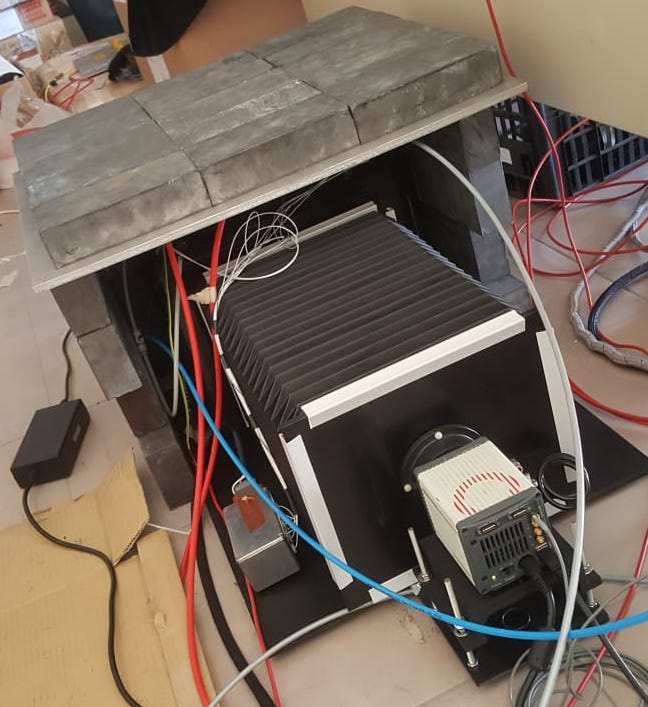
\includegraphics[width=0.45\linewidth]{LEMON-Shielded.jpg}
  	\caption{\lemon with the lead shield of the  drift volume cage. The sCMOS camera (on the front) is looking at the GEMs through a blackened bellow.}
  	\label{fig:LemonShielded}
\end{figure}



Typical images frame obtained with a 30 ms exposure time of the sCMOS
camera are shown in Fig.~\ref{fig:typicalimage1}. Several light spots
are visible due to different ionization patterns due to different types of particles interacting in the
gas.   Fig.~\ref{fig:typicalimage1} (left) shows an
image with typical long tracks from cosmic rays travelling through the
full gas volume, where clusters of light with larger  energy deposition are
clearly visible, superimposed to  radioactivity events likely due to natural origin.
Fig.~\ref{fig:typicalimage1} (right) shows an example of a cleaner event
with one straight cosmic ray track, that can be used for energy
calibration purposes.

The events shown in Fig.~\ref{fig:signals} show images recorded with
the same 30 ms exposure time, but in presence of radioactive
sources. Figure~\ref{fig:signals} (left) shows one example of several
energy spots, characteristic of 5.9 keV energy deposits of a  \fe
radioactive $\gamma$-source.  This is the standard candle for calibration and
performance evaluation of \lemon, and its extensive use is documented in
Ref.~\cite{bib:fe55}. Figure~\ref{fig:signals} (right) shows an event
recorded in presence of the \ambe radioactive source, which emits neutrons in the 
$\alpha \, ^{9}Be \rightarrow \, n ^{12}C  \, \gamma$ reaction. 

 
\begin{figure}[ht]
  \begin{center}
    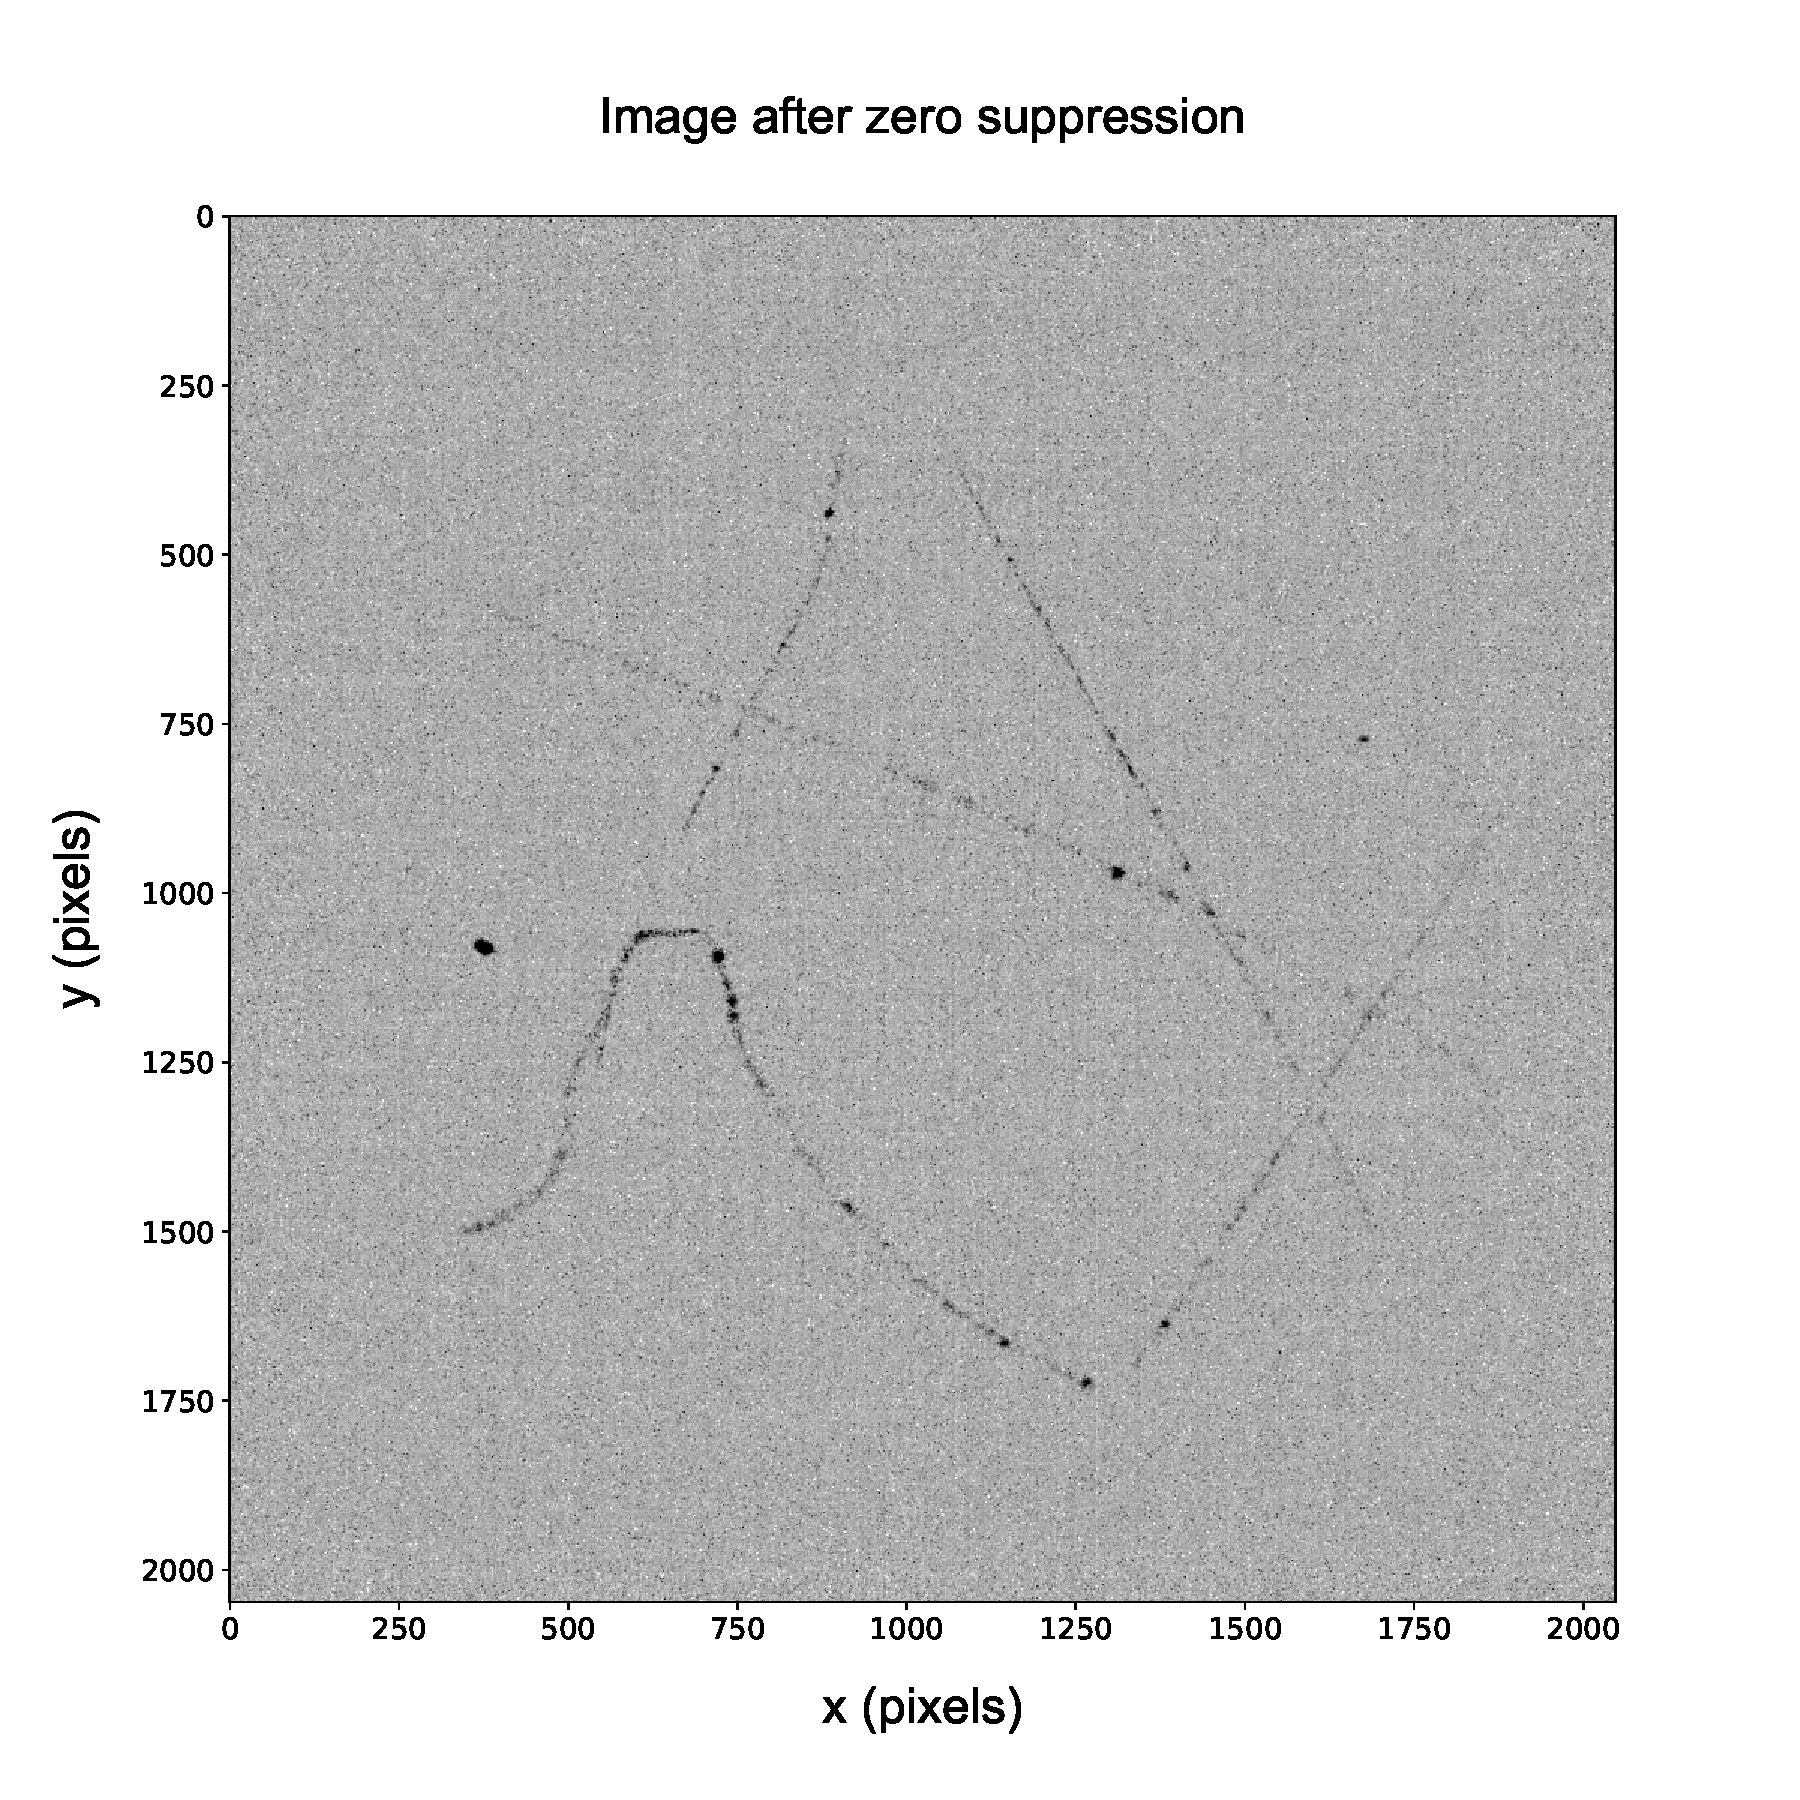
\includegraphics[width=0.49\linewidth]{figures/pic_run02317_ev8_oriIma_paper}
    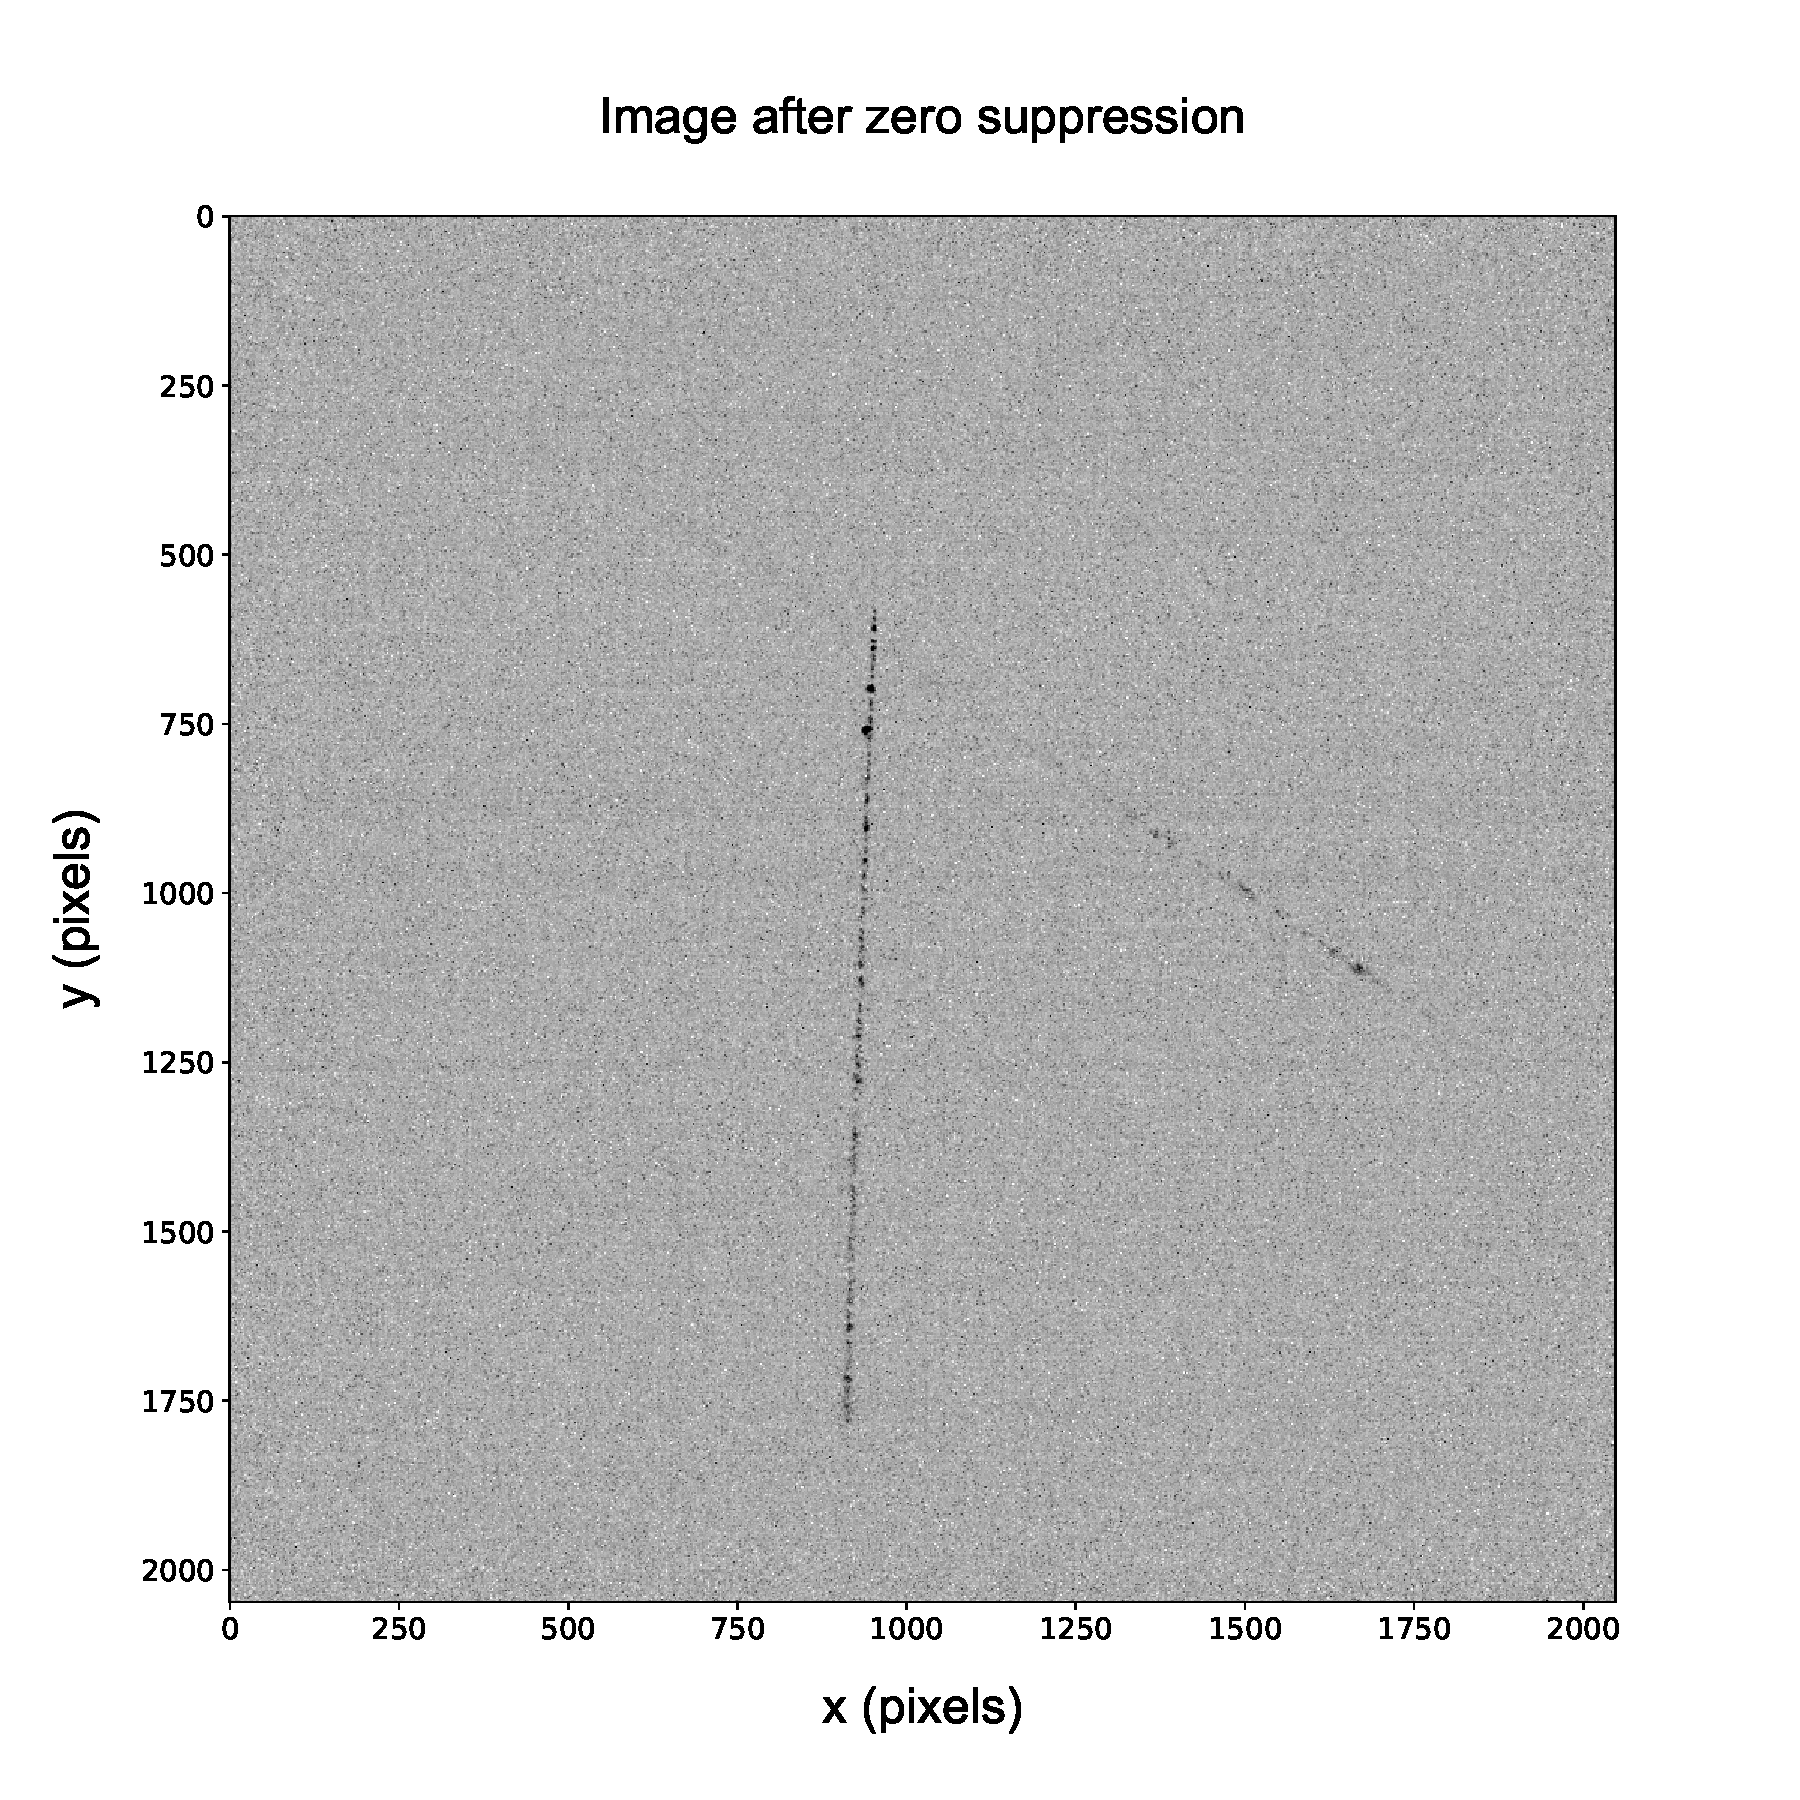
\includegraphics[width=0.49\linewidth]{figures/pic_run02156_ev527_oriIma_paper}
    \caption{Two typical pictures taken with the sCMOS camera with a 30
      ms exposure time. Left: cosmic tracks and natural radioactivity
      signals are present. Right: two long cosmic rays tracks are
      present, observed in a run without any source.
      \label{fig:typicalimage1}}
  \end{center}
\end{figure}

 
\begin{figure}[ht]
  \begin{center}
    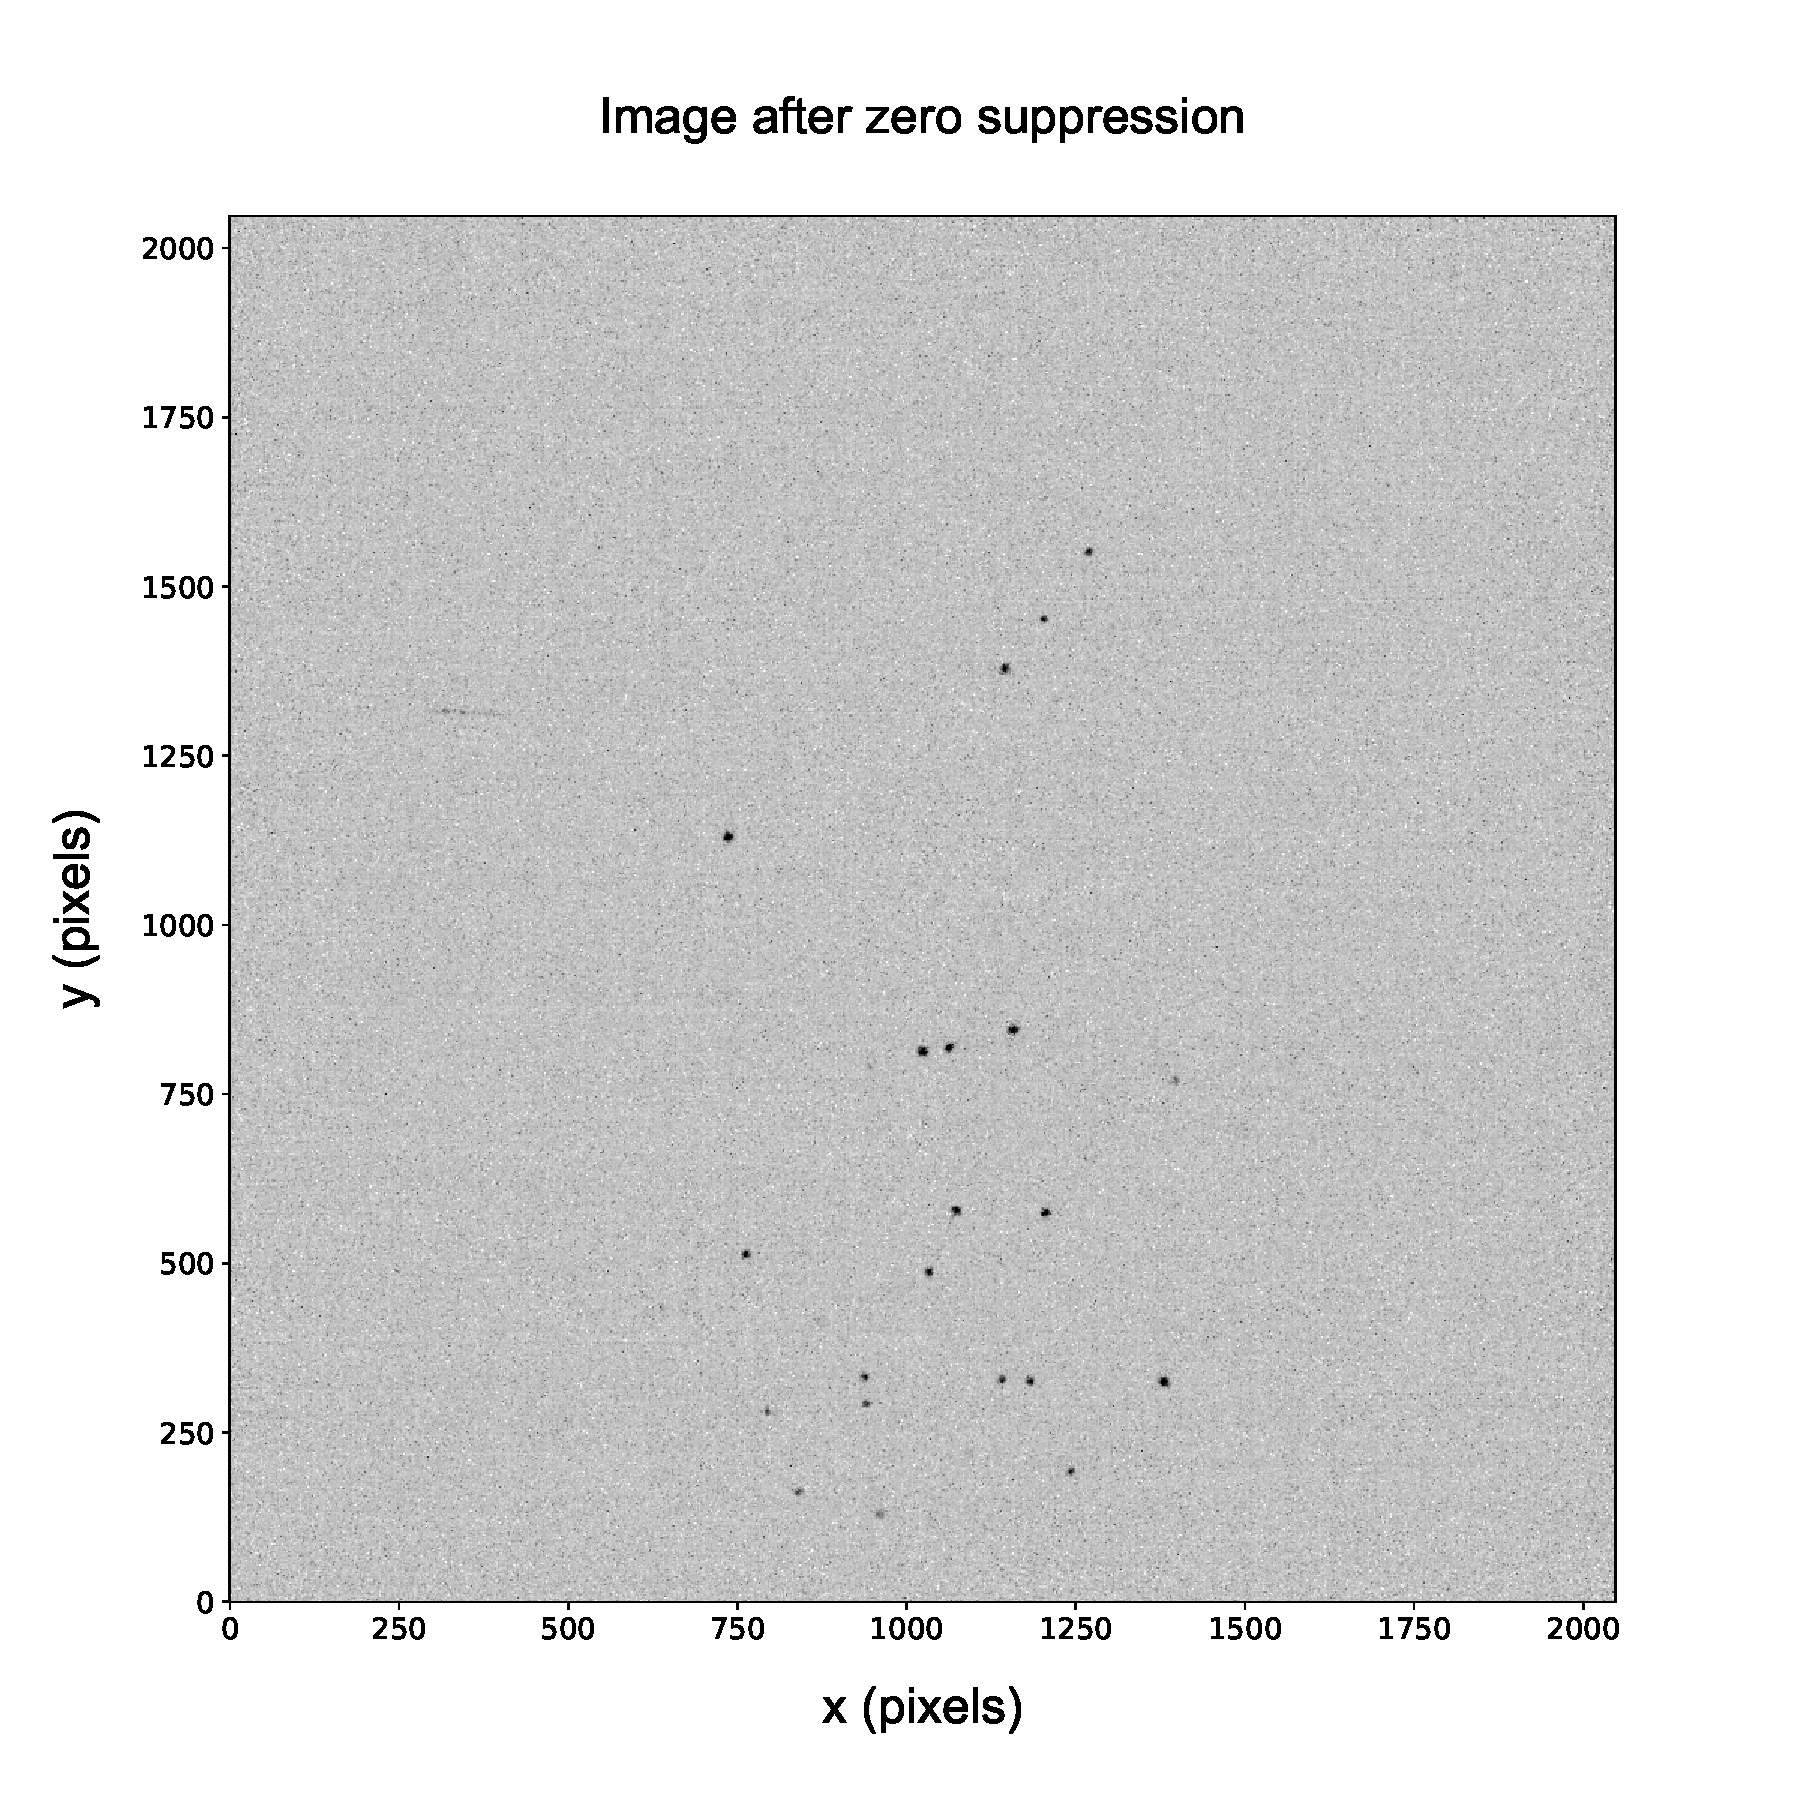
\includegraphics[width=0.49\linewidth]{figures/pic_run01843_ev93_oriIma_paper}
    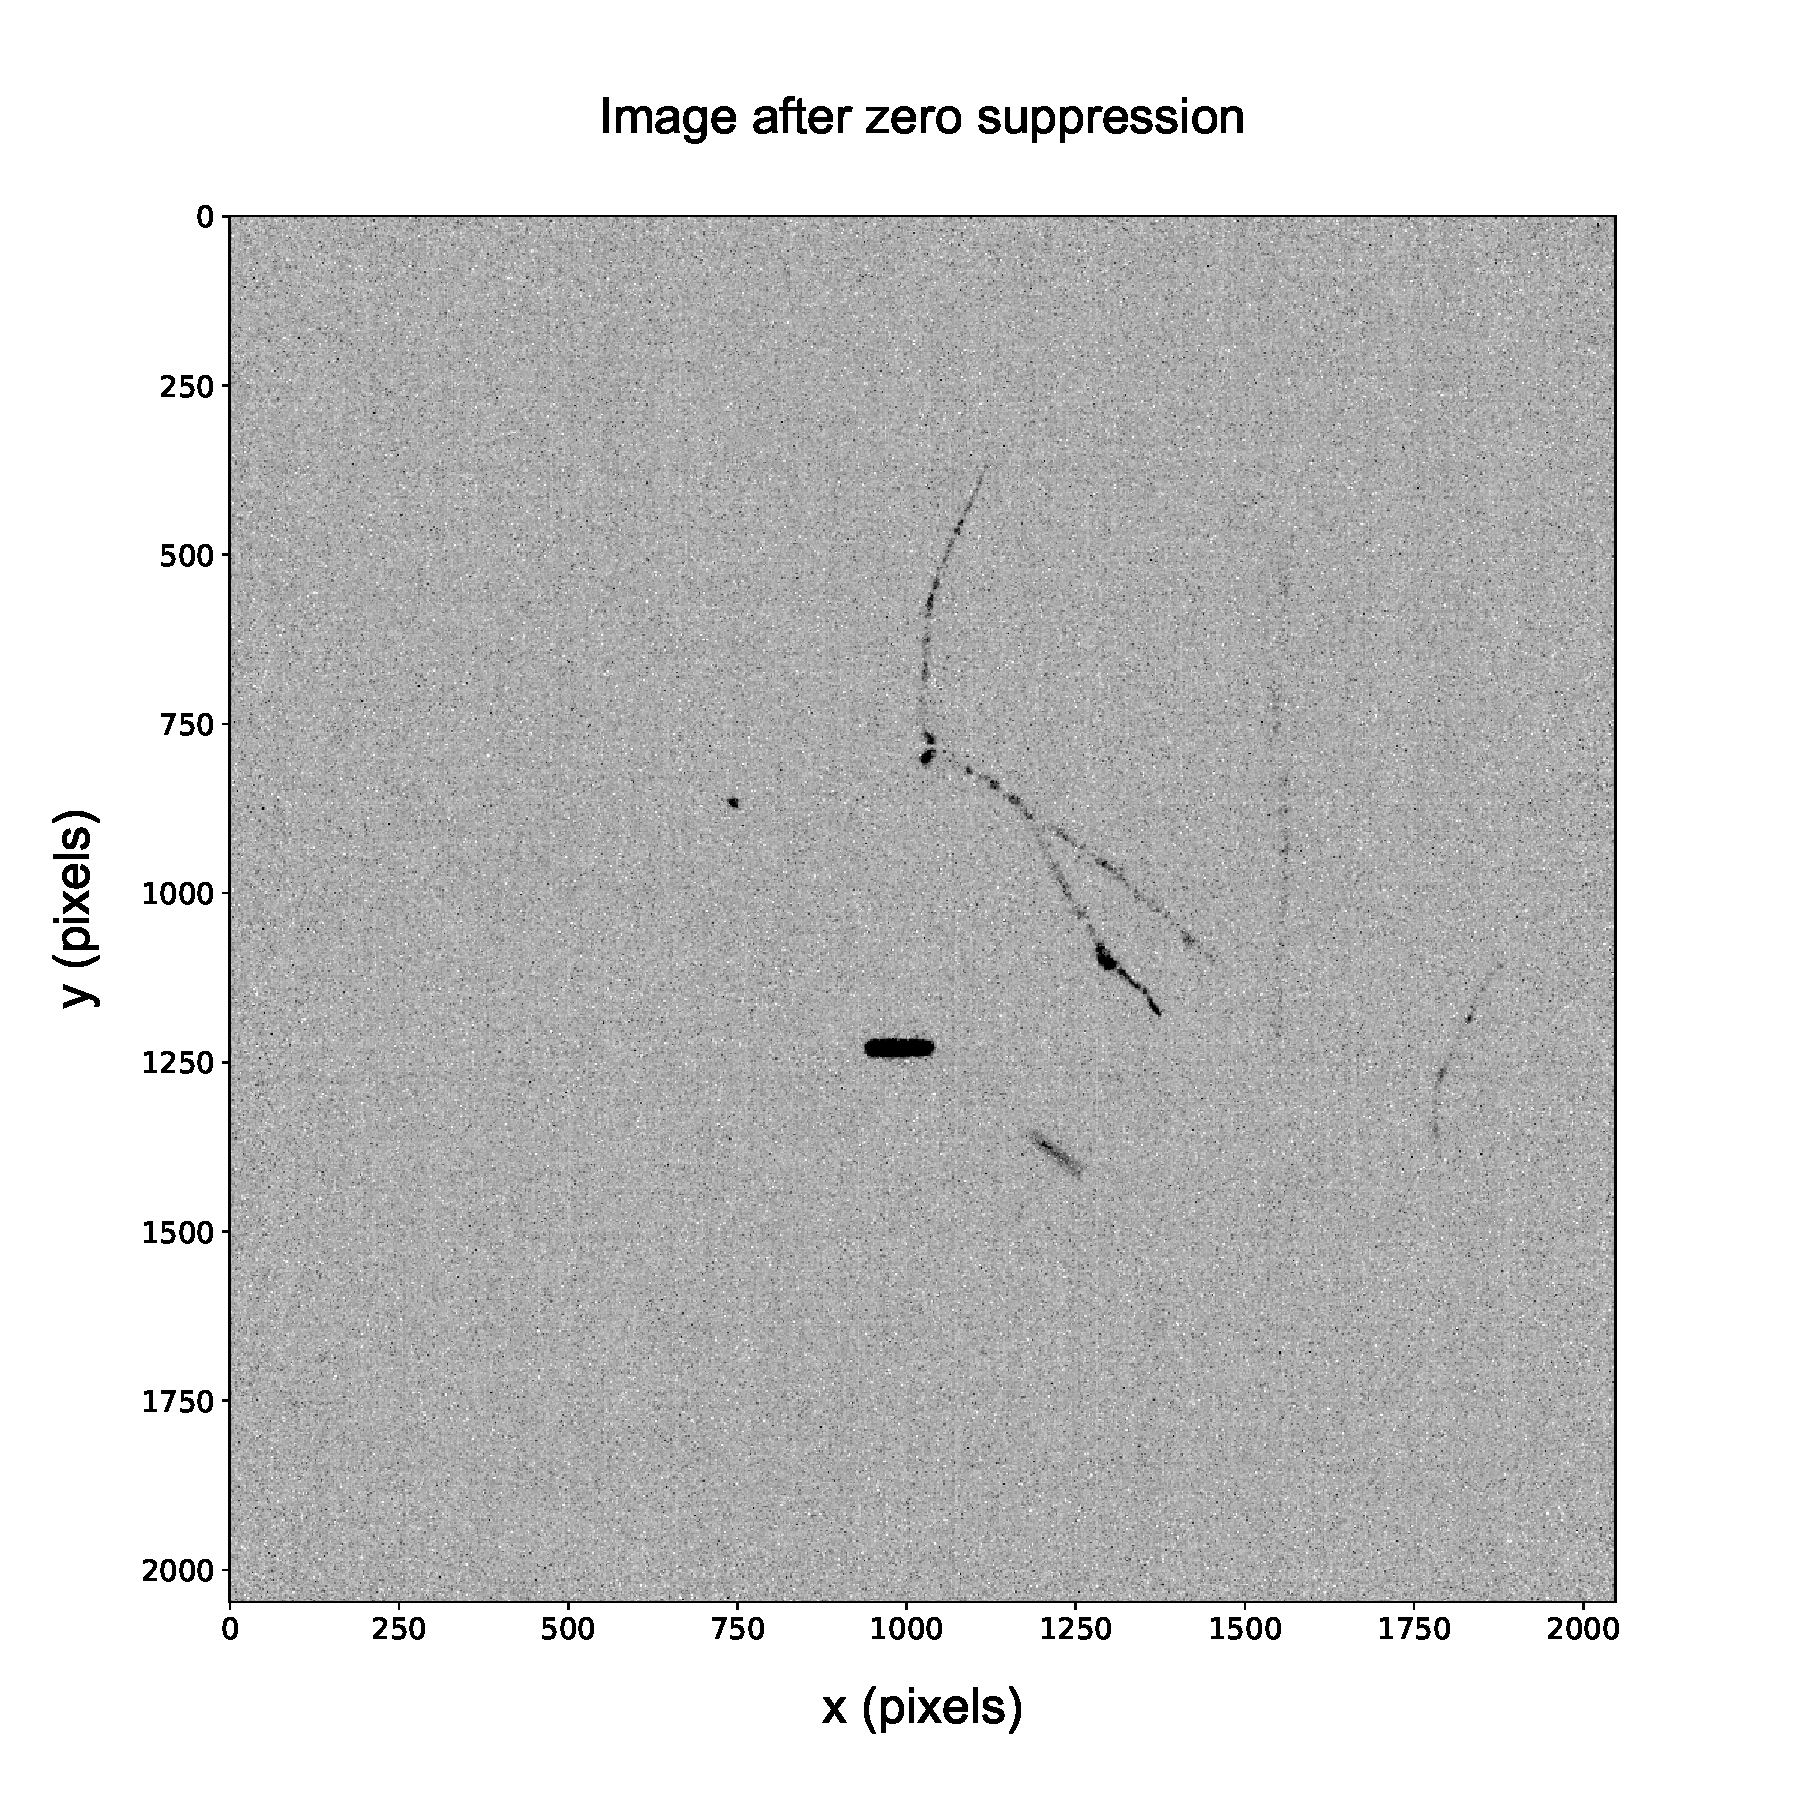
\includegraphics[width=0.49\linewidth]{figures/pic_run02317_ev342_oriIma_paper}
    \caption{Two pictures taken with the sCMOS camera with a 30 ms
      exposure time. Left: picture taken in presence of \fe radioactive
      source. Right: a nuclear recoil candidate is present, in an image
      with \ambe radioactive source, together with signals from natural
      radioactivity.      \label{fig:signals}}
  \end{center}
\end{figure}

\lemon was operated in an overground location at Laboratori Nazionali di Frascati (LNF) with  a He-CF$_4$ (60/40) gas mixture, the triple GEM system set at a voltage across the GEM sides of \textcolor{red}{xxx~V} and an electric field between them of \textcolor{red}{x.0} kV/cm - using a HV GEM power supply \cite{Corradi:2007df} ensuring stability and accurate monitoring of the bias currents. The gas mixture was kept at atmospheric pressure under continuous flow of about \textcolor{red}{x.0} cc/min and with the GEMs operated at \textcolor{red}{x.0} $ \times10^5$ gain. The typical photon yield for this  type of gas mixtures has been measured to be around  0.07 photons per avalanche electron.\cite{bib:jinst_orange1, bib:roby, bib:tesinatalia}

The field cage was powered by a CAEN N1570.\cite{CAENN1570} generating an electric field  of 0.6 kV/cm. 

\textcolor{red}{this part was copied by the lemon btf paper - must be revised}
\textcolor{red}{The ORCA Camera I/O has been configured in order to get a pre-trigger, that must occur 80~$\mu$s before the shutter, and to synchronize the PMT signal waveform acquired with an oscilloscope LeCroy 610Zi. Optics and exposure time (30~ms) were optimized to ensure the largest light collection and to avoid events due to the natural radioactivity. Between 100 and 300 images were typically acquired per run. }

A  5cm thick lead shielding was mounted around the \lemon field cage to reduce the natural radioactivity background. From the measurements of the GEM current with and without the lead shielding a reduction of a factor 2  of the total ionization in the sensitive volume  - very likely due to external radioactivity -  was estimated.

 An neutron source, based on a 3.5~$\times~$10$^3$~MBq activity  $^{241}$Am source contained in a Beryllium capsule (\ambe) was placed at a distance of 50~cm from the sensitive volume side. 
 Because of the interactions between $\alpha$ particles produced by the $^{241}$Am and the Beryllium nucluei, the \ambe source isotropically emits:
 \begin{itemize}
     \item photons with an energy of 59~keV produced by $^{241}$Am;
     \item neutrons with a kinetic energy mainly in a range between 1 to 10 MeV;
     \item photons with an energy of 4~MeV produced along with neutrons in the interaction between $\alpha$ and Be nucleus.
 \end{itemize}
 
The presence of a lead shield around the sensitive volume absorbed almost completely the 59~keV photon component. A small faction of them reached the gas through small gaps accidentally present between the bricks.
 

\clearpage
 
\section{Cluster pattern recognition}
\label{sec:clustering}
The light produced in the multiplication process in the GEM and
detected by the CMOS sensor is associated in clusters of neighboring
pixels. This is done by following the trail of energy deposition of the particle travelling
through the gas of the sensitive volume. The deposited energy  (that for stopped particles is equivalent to the total energy of the particle)
 is estimated by the amount of the light
collected by the sensor.  Therefore, it is of primary importance to
have a reconstruction algorithm that  includes all  the pixels
hit by the real photons originating from the energy deposits, while
rejecting most of the electronic noise. This can either create fake
clusters or, more likely, add pixels in the periphery of clusters from
real photons, biasing the energy estimate.

The energy reconstruction follows a three-steps procedure: the
single-pixel noise suppression is briefly described in
Section~\ref{sec:zerosuppression}. This is followed by the proper  clustering: first the basic clusters of single small deposits is
described in Section~\ref{sec:basiccl}, then the superclusters, aiming
to follow the track patterns for depositions extended in space, and
seeded by the basic clusters, is described in
Section~\ref{sec:supercl}.

The results of this paper are based on the properties of the
reconstructed superclusters and are described in
Section~\ref{sec:clustershapes}.


\subsection{Noise suppression}
\label{sec:zerosuppression}
The electronic noise of the sensor is estimated in runs acquired
with the sensor in complete dark ({\it pedestal} runs). For each
pixel, the pedestal is computed as the average of the counts over many
events \textcolor{red}{non sarebbe meglio chiamarli frames ? o images ? }, while the electronic noise is computed as the standard deviation
(SD) of the counts. The distribution of the pixels SD is shown in
Fig.~\ref{fig:noise}. The mode of this distribution is about 1.8
photons per pixels, but a tail is present, with pixels having a
 noise of more than 5 photons per pixels.
The pedestal $\mu_i$ is then subtracted to the image for each $i^th$ pixel.
An initial noise suppression is applied by neglecting the pixels with counts less than $1.3\times\textrm{SD}_i$.
%where $i$ represents the
%pixel (\textit{zero suppression}). 
%
\begin{figure}[ht]
  \centering
  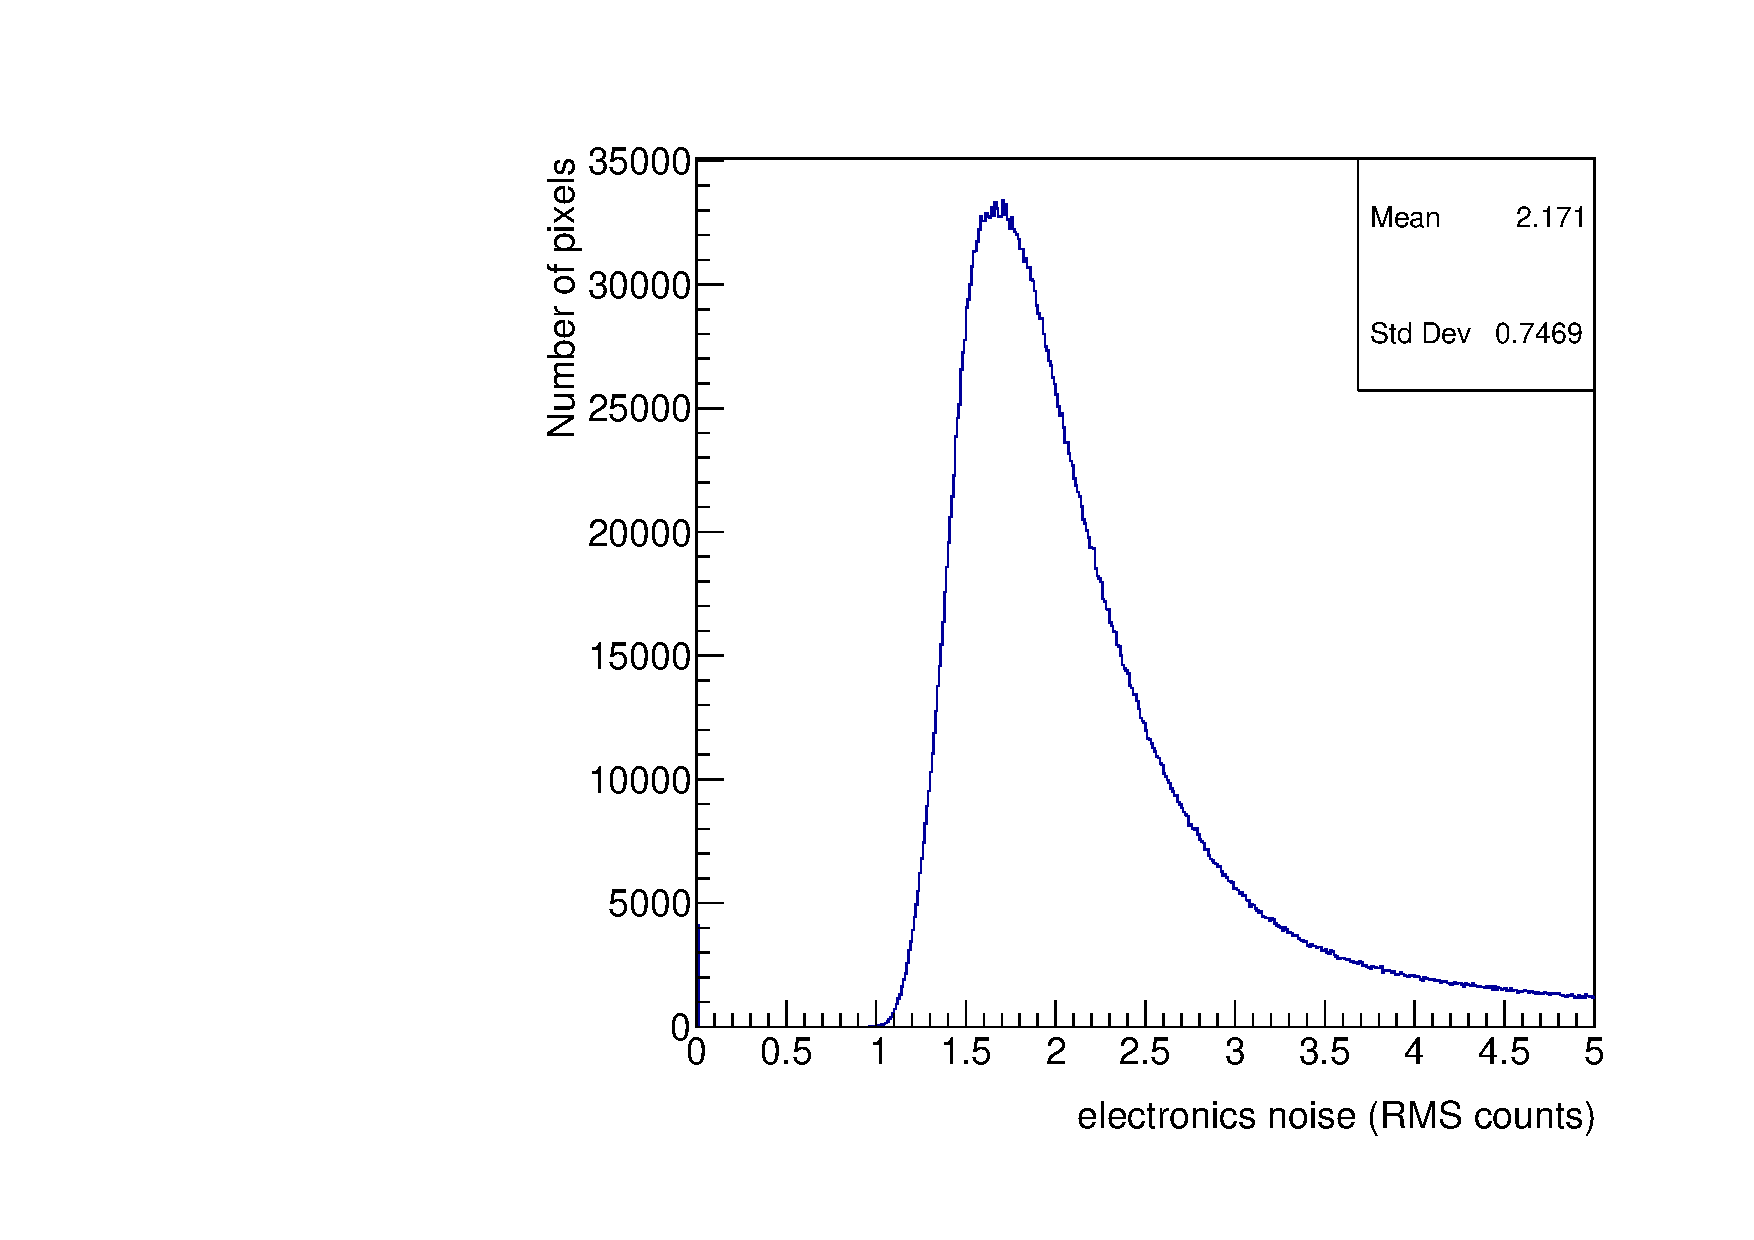
\includegraphics[width=0.45\linewidth]{figures/sensor_noise}
  \caption{Distribution of the electronic noise of the sensor,
    estimated in images taken with sensor in complete dark, and
    evaluated as the RMS of the distribution of the counts for each
    pixel.  \label{fig:noise}}
\end{figure}
%
On such pedestal-subtracted zero-suppressed images  an upper
threshold is applied to reject hot pixels, which are more likely due
to sensor instabilities than to energy deposition. These are not
malfunctional pixels  because they disappear after a
power cycle of the camera and therfore a dynamic (run-by-run) suppression is
needed.  The hot pixels are efficiently identified as high-intensity, isolated
pixels, and distinguished by a true energy deposit, for which each
pixel is surrounded by some other active pixels. A minimum average of
the counts, and a minimum number of two pixels above noise in a
$3\times3$ pixels matrix surrounding the hot pixel is required.
\textcolor{red}{is required to do what ? to retain the pixel ?}

The resolution of the resulting image is then reduced by creating
\textit{macro-pixels}, by averaging the counts in $4\times4$ pixel
matrices. This is needed to reduce the combinatorics   of the following
clustering algorithm to be executed   in a reasonable time for each
image. On such $512\times512$ pixel map, a median
filtering~\cite{medianfilter} is applied, as described in more details
in Ref.~\cite{medianfilter_cygno}. The output image is passed to the
basic clustering algorithm, described in the following.





\subsection{Basic clusters reconstruction}
\label{sec:basiccl}
The basic clustering algorithm is described in full details in
Ref.~\cite{iDBSCAN}, and it is briefly summarized here.
The energy deposition pattern in the active volume of the TPC,
and thus its two-dimensional (2D) projection on the $x--y$ axes 



\subsection{Super clusters reconstruction}
\label{sec:supercl}
The aim of the superclustering procedure is to collect the majority of
the pixels belonging to a track which is longer and possibly with a
pattern more irregular than the one clustered by \idbscan. The main
limitation of \idbscan to follow a long track is mainly originated by
the irregular behavior of the energy deposition along the path length.
As can be clearly seen in Fig.~\ref{fig:basic_clusters} (right), or
even in the example of a raw image of an event with two long cosmic
rays in Fig.~\ref{fig:typicalimage1} (right), clusters with larger
energy release are followed by regions along the path with a lower or
even a zero release.  These local minima are sometimes as large, in
the 2D space, as the typical size of the $\epsilon$ parameter of
\dbscan~\cite{dbscan}. Despite the low electronic noise of the
ORCA-Flash 4.0 camera sensor, the energy releases in these local
minima are similar in magnitude to the average single-pixel noise.
The \idbscan is limited in connecting the full length of an extended
path, because of two reasons. First, inflating $\epsilon$ parameter as
much as needed to cover the areas of local minima conflicts with the
need to reject noise around the cluster.  The \idbscan parameters are
optimized for the \lemon running conditions to collect most of the
signals of $E \approx 5$\keV and rejecting the typical noise of
$\approx 1$ photon per pixel. This avoids collecting extra noise in
the cluster, biasing the energy scale and worsening its resolution,
and keeps the rate of fake clusters at a negligible level.  This is
studied in great detail in Ref.~\cite{iDBSCAN}.  Second, the iterative
nature of the algorithm with very different parameters for each
iteration, each tuned for very different intensity, makes it
convenient and efficient for a deposition of a fixed energy density
(like the spots originating from the \fe source), but not for the cases
like the Fig.~\ref{fig:basic_clusters} (right), where the same track
is split in several parts, with some of them in different iterations.
This requires a method that can continuously follow the pattern of the
track, profiting of the full resolution image, where the {\it gradients} of
the energy deposition along the track trajectory are smaller than the
ones in the transverse direction. Running any of the most common
methods on the full $1024\times1024$ image is not manageable CPU-wise,
due to huge combinatorics while maintaining the limited zero-suppression
described previously.

The procedure adopted for the final supercluster reconstruction in the
\lemon detector starts from defining the \textit{interesting regions}
in the image that may contain pixels from an energy deposit. These are
identified by the basic cluster algorithm \idbscan previously
described and run \textcolor{red}{run ??} in the $512\times512$
reduced-resolution image. In order to gather the peripheral pixels,
especially along the track trajectory where breaks in sub-basic
clusters may have happened, a window of $5\times5$ pixels is
considered, around each pixel belonging to a macro-pixel clustered in
a basic cluster. A full resolution image formed only by the
interesting pixels passing the simple initial filtering described in
Sec.~\ref{sec:zerosuppression} is formed.  The gradients of such image
are computed pixel-by-pixels to look for the edge region where the
image changes from signal to noise-only:
\begin{equation}
\label{eq:gradient}
\vert\vert\nabla(N)\vert\vert =
\sqrt{\left(\frac{\partial N}{\partial x}\right)^2
  +\left(\frac{\partial N}{\partial y}\right)^2},
\end{equation}
and the gradient direction is given by:
\begin{equation}
  \label{eq:graddir}
  \theta = \tan^{-1}\left(\frac{\partial N}{\partial y}/\frac{\partial N}{\partial x}\right).
\end{equation}
In order to reduce the effect of the noise which makes the first
derivatives in Eq.~\ref{eq:gradient} to fluctuate, a Gaussian
filtering is applied, with a 5$\sigma$ threshold, where $\sigma$ is
the standard deviation of the intensities of the pixels considered.

After this filtering is applied, the superclustering algorithm is an
application of the \textit{morphological geodesic active
  contours}\cite{gac,mgac}, called \gac in the following.  This method
us an active contour finding algorithm, widely used in computer
vision, where the boundary curve $\mathcal{C}$ of an object is
detected by minimizing the \textit{energy} associated to $\mathcal{C}$:
\begin{equation}
  \label{eq:gacenergy}
  E(\mathcal{C}) = \int_{0}^{1} g(N)(\mathcal{C}(p)) \cdot \vert\mathcal{C}_p\vert dp,
\end{equation}
where $N$ is the number of photons in the pixel (intensity), $ds=
\vert\mathcal{C}_p\vert dp$ is the arc-length parametrization of the
curve in the 2D space, and $g$ is the stopping edge function, which
allows to select the boundary of the cluster.  In the \gac method used
here, the $g$ function is purely geometrical, and uses geodesics of
the image, \ie, local minimal distance path between points with the
same gradient, defined before. The function $g(N)$ is given by:
\begin{equation}
g(N) = \frac{1}{\sqrt{1+\alpha\vert\nabla G_\sigma * N\vert}},
\end{equation}
which is minimal in the edges of the image.  The $G_\sigma * N$ is the
aforementioned Gaussian filter with standard deviation $\sigma=5$, and
the parameter $\alpha$, which regulates the strength of the filtering
is tuned on typical \lemon images to be $\alpha=100$.

This method has been chosen because it allows to follow track patterns
that may vary from convex to concave shape, and also have kinks, in
cases of $\delta$-rays. To improve the shrinking of the cluster
boundary in the cases of concave-convex tracks, the \textit{balloon}
force~\cite{mgac} is set to -1, in order to push the contour towards a
border in the areas where the gradient is too small. A number of 300
iterations is used to evolve the supercluster contour.

The supercluster obtained on the same track shown in
Fig.~\ref{fig:basic_clusters} (right) after the basic clustering step,
is shown again in full resolution, zoomed around the cluster, in
Fig.~\ref{fig:super_clusters1} (left). The output of the
superclustering with the \gac algorithm is shown on the rihgt panel of
the same figure. The splitting of the clustering present after the
basic cluster step has been recovered, and sections with high density
and low density along the path of the energy deposition have been
joined. Other three examples of superclustered images are shown in
Fig.~\ref{fig:super_clusters2}, in runs without any radioactive
source. The top left panel shows an example of a cosmic ray track
fully reconstructed by the \gac superclustering, which also includes a
$\delta$-ray in the middle of the track length. The top right panel shows an
example of curly track from a candidate of natural radioactivity
interaction; bottom panel shows an example where both a cosmic ray and
a curly track are present. In this case, the extremes of the long and
straight track are still split, but this is much rarer than with the
basic clustering, and it happens when the local minimal along the
trajectories are compatible with noise-only for more than
$\approx$1\unit{cm}.
%
\begin{figure}[ht]
  \begin{center}
     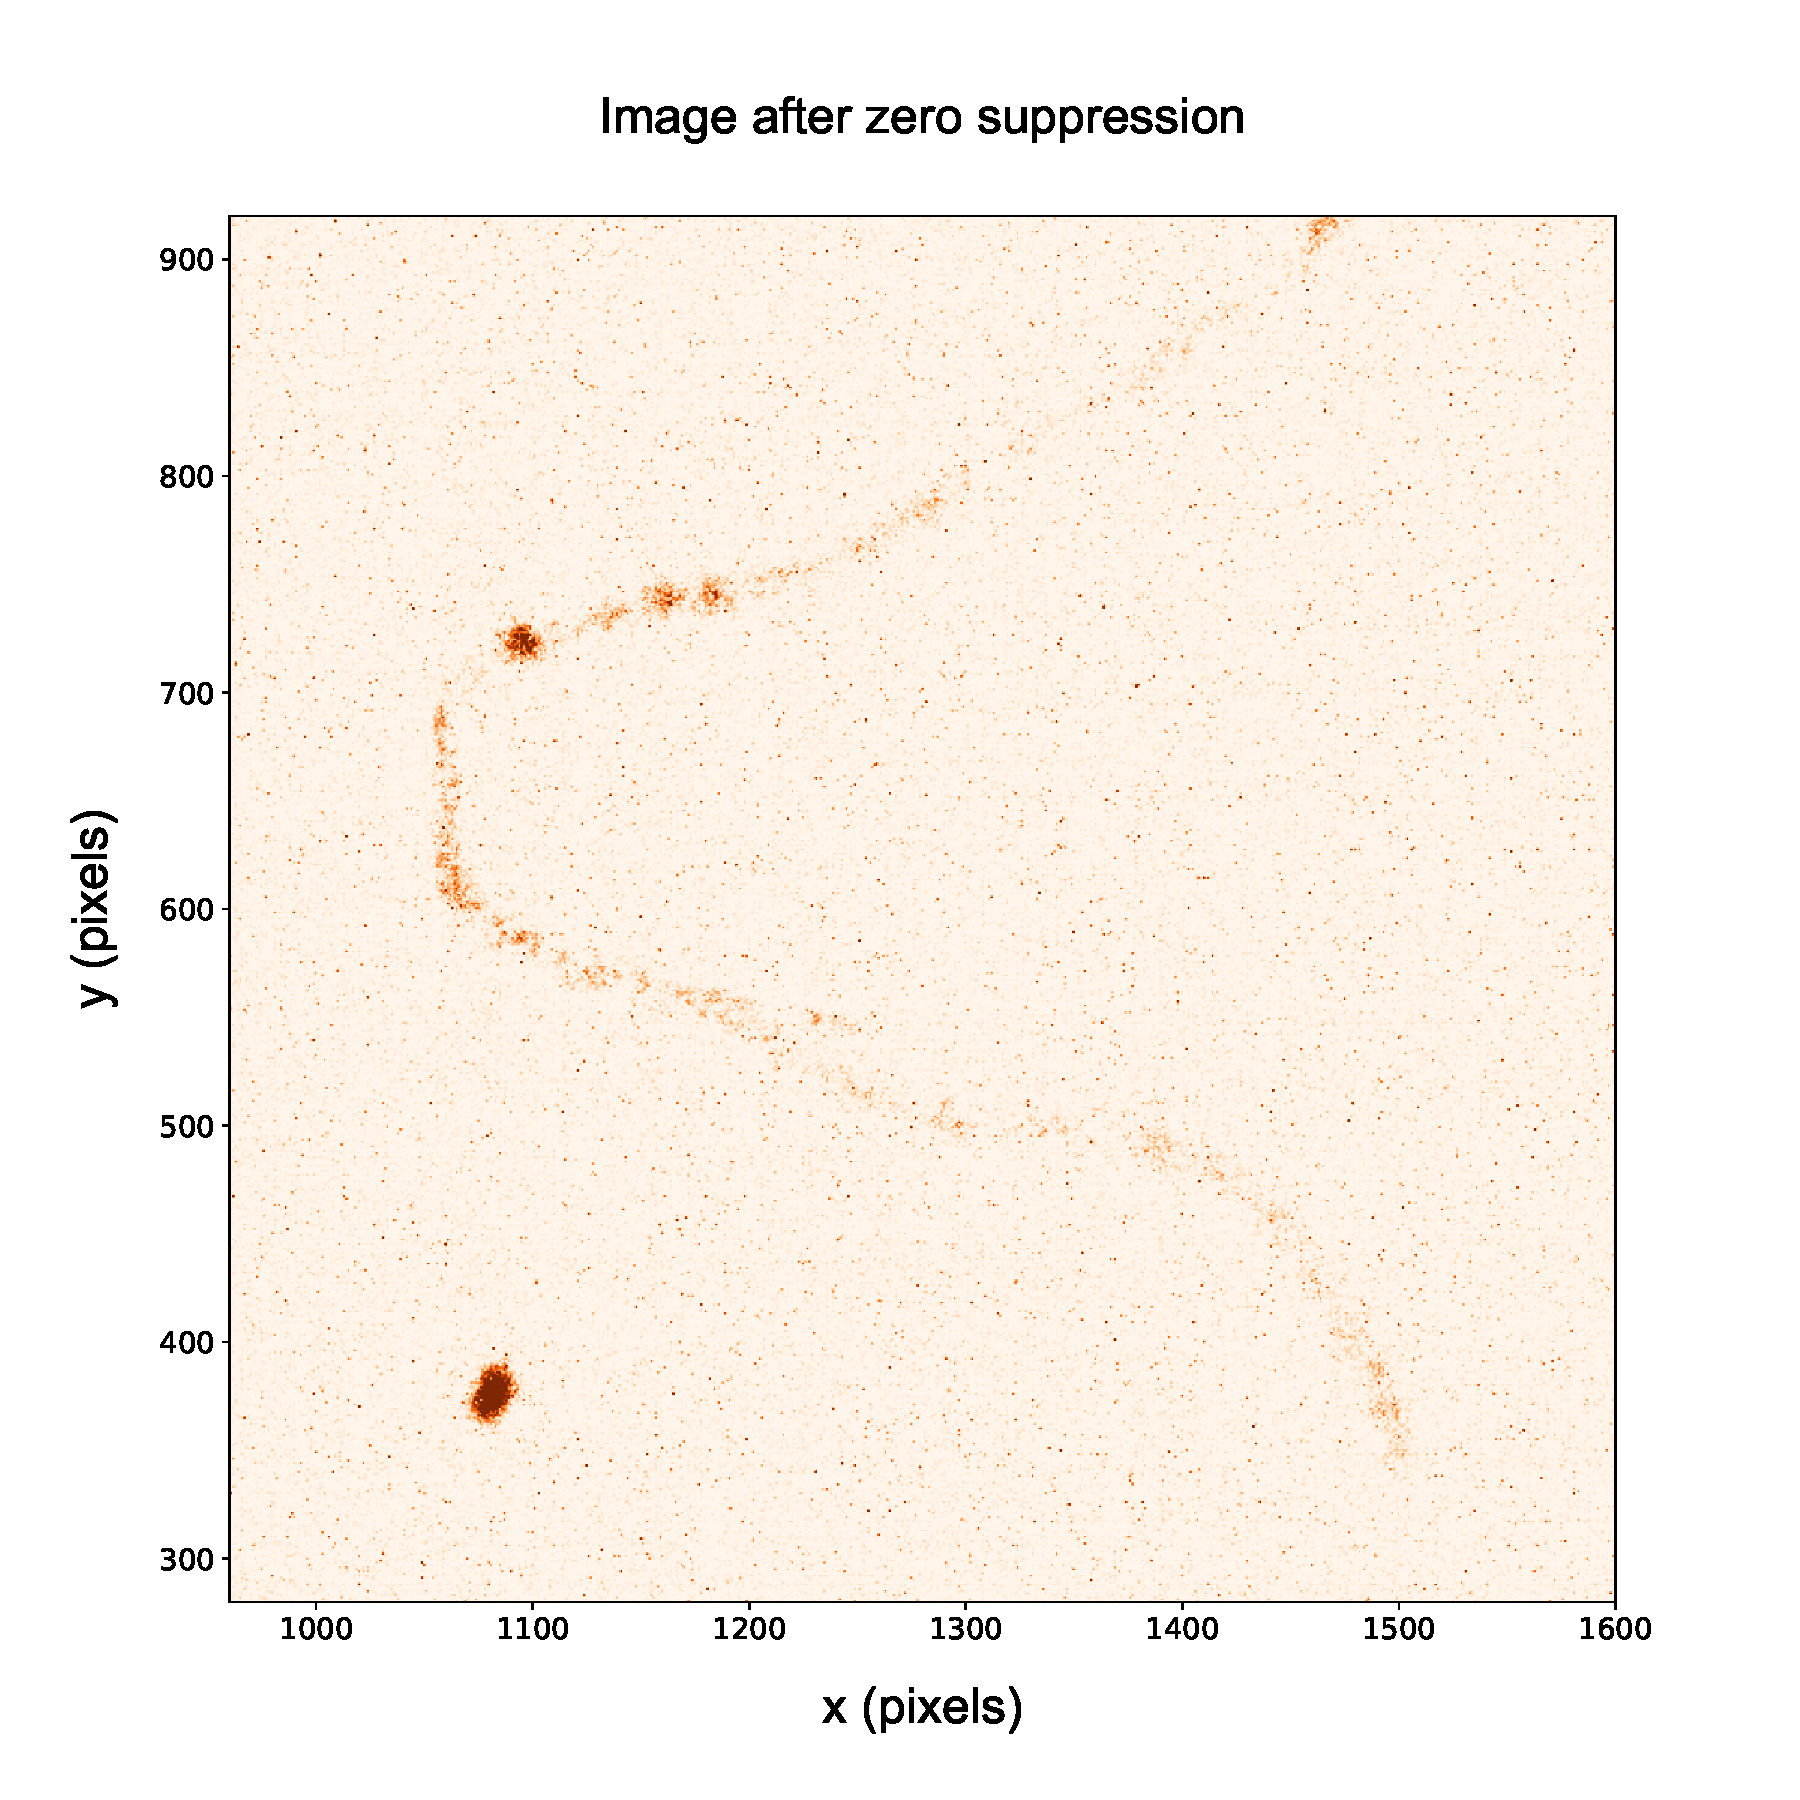
\includegraphics[width=0.49\linewidth]{figures/pic_run02317_ev8_oriIma_paper_zoom}
      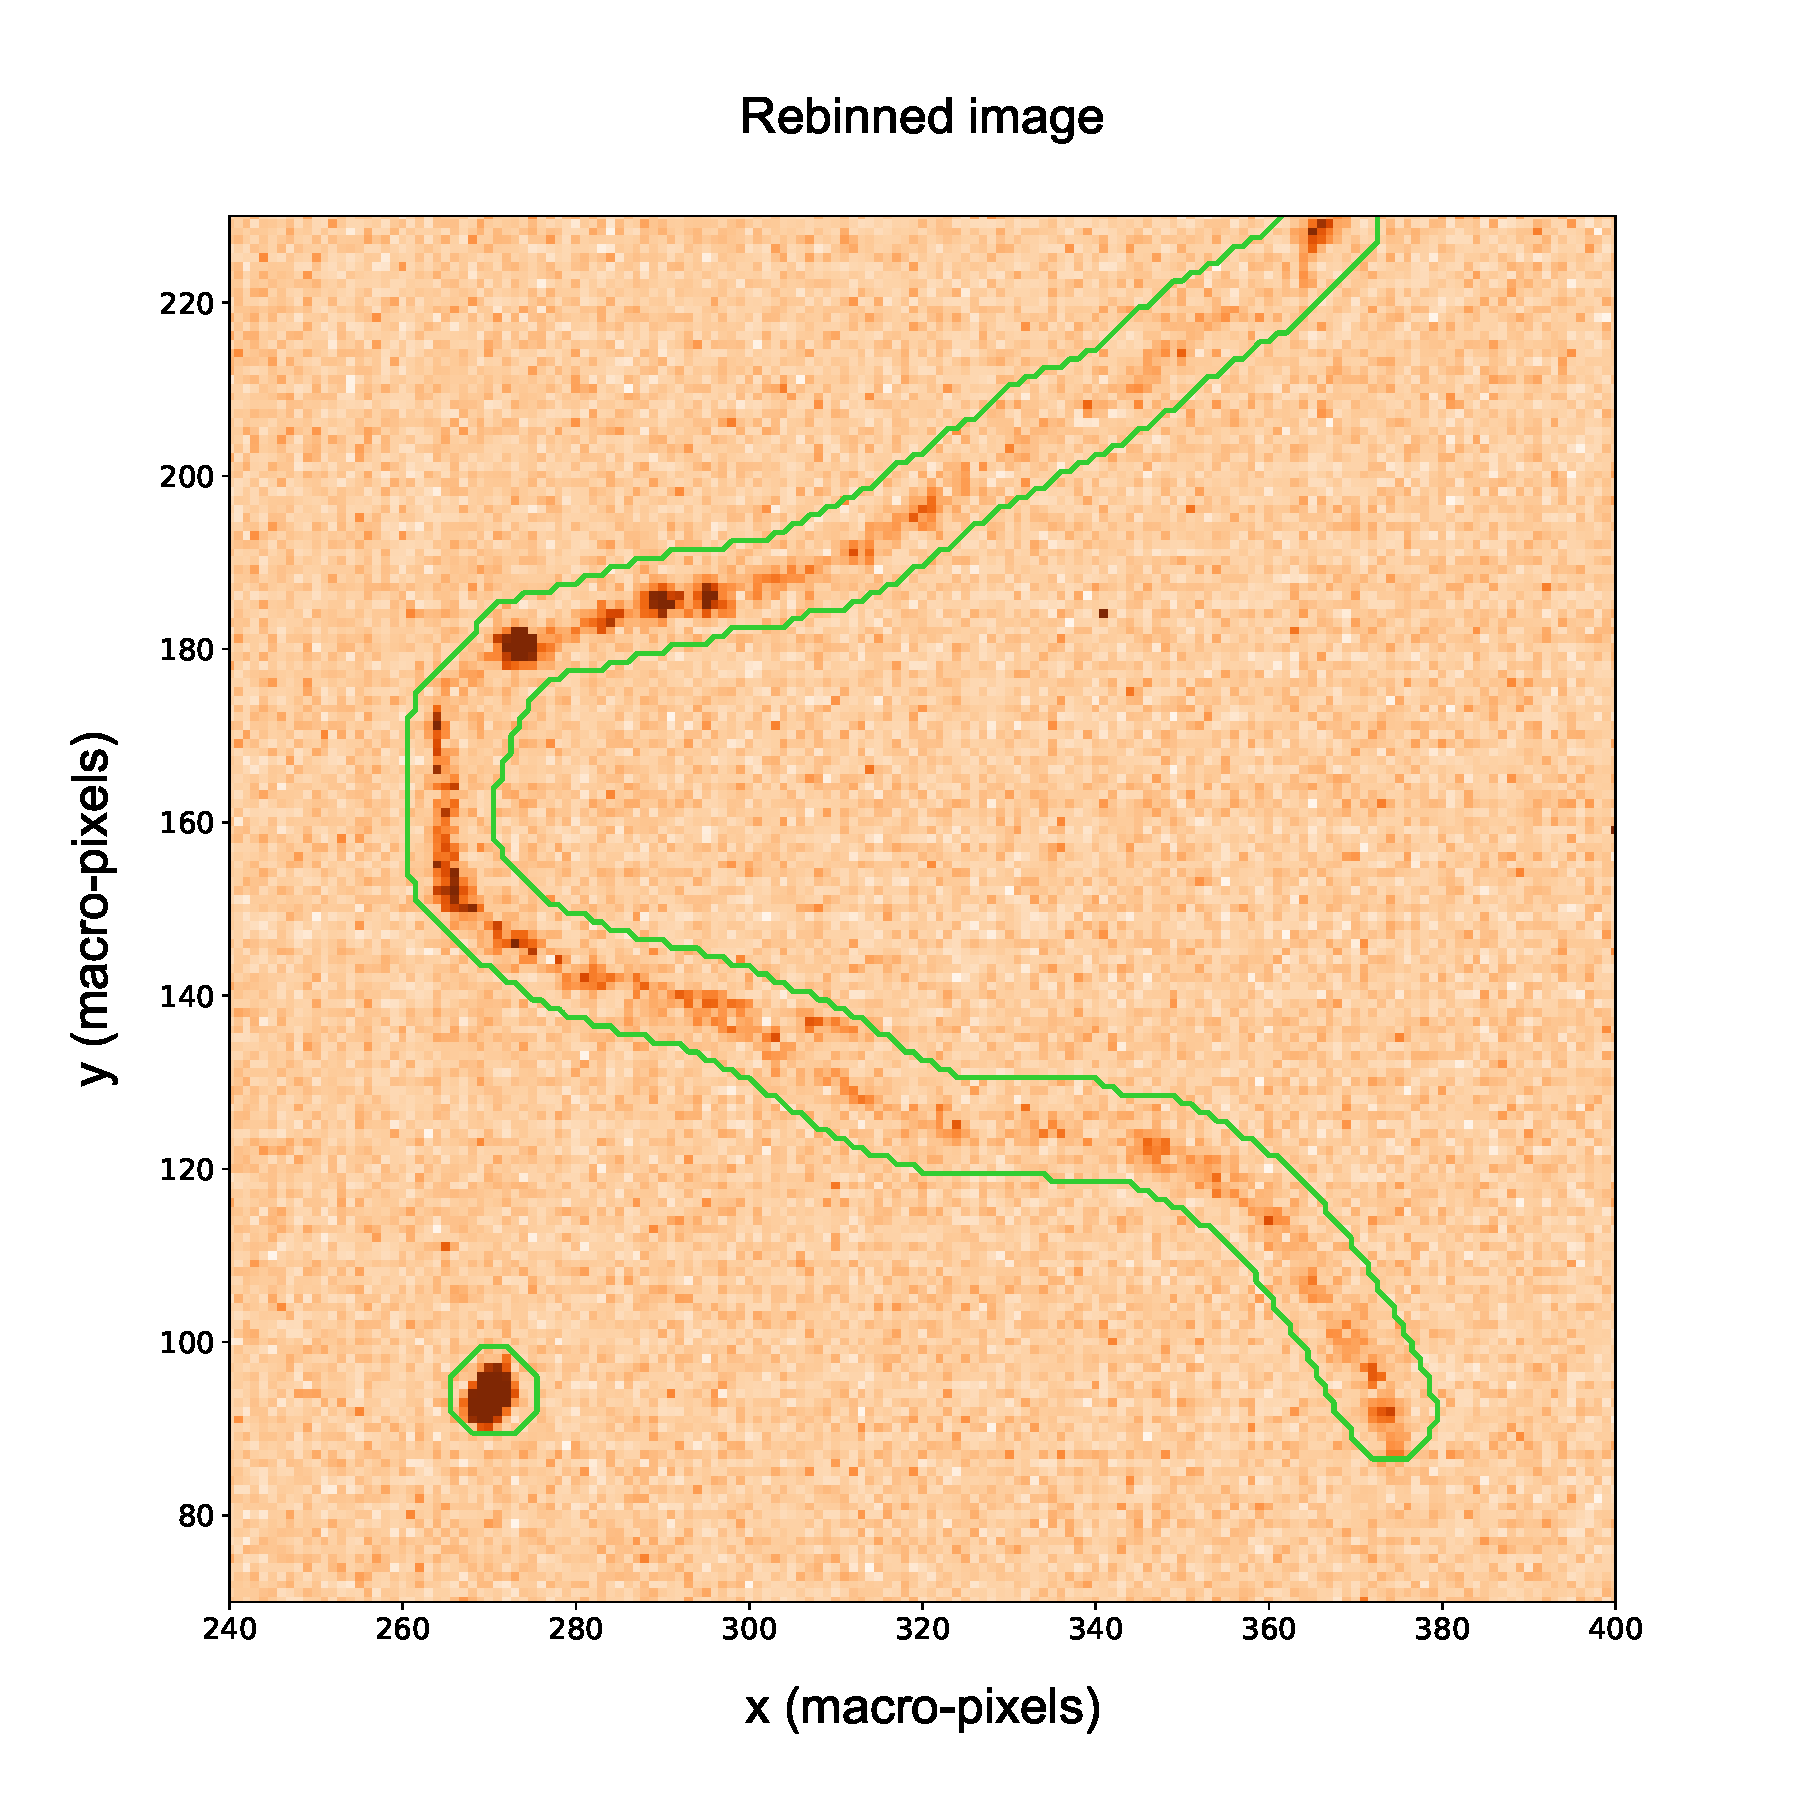
\includegraphics[width=0.49\linewidth]{figures/pic_run02317_ev8_sc_3D_paper}
      \caption{Left: zoom on the full-resolution image of a
        track candidate in a run with \ambe radioactive
        source. Right: output of the superclustering on the rebinned
        image. \label{fig:super_clusters1}}
  \end{center}
\end{figure}
%
\begin{figure}[ht]
  \begin{center}
     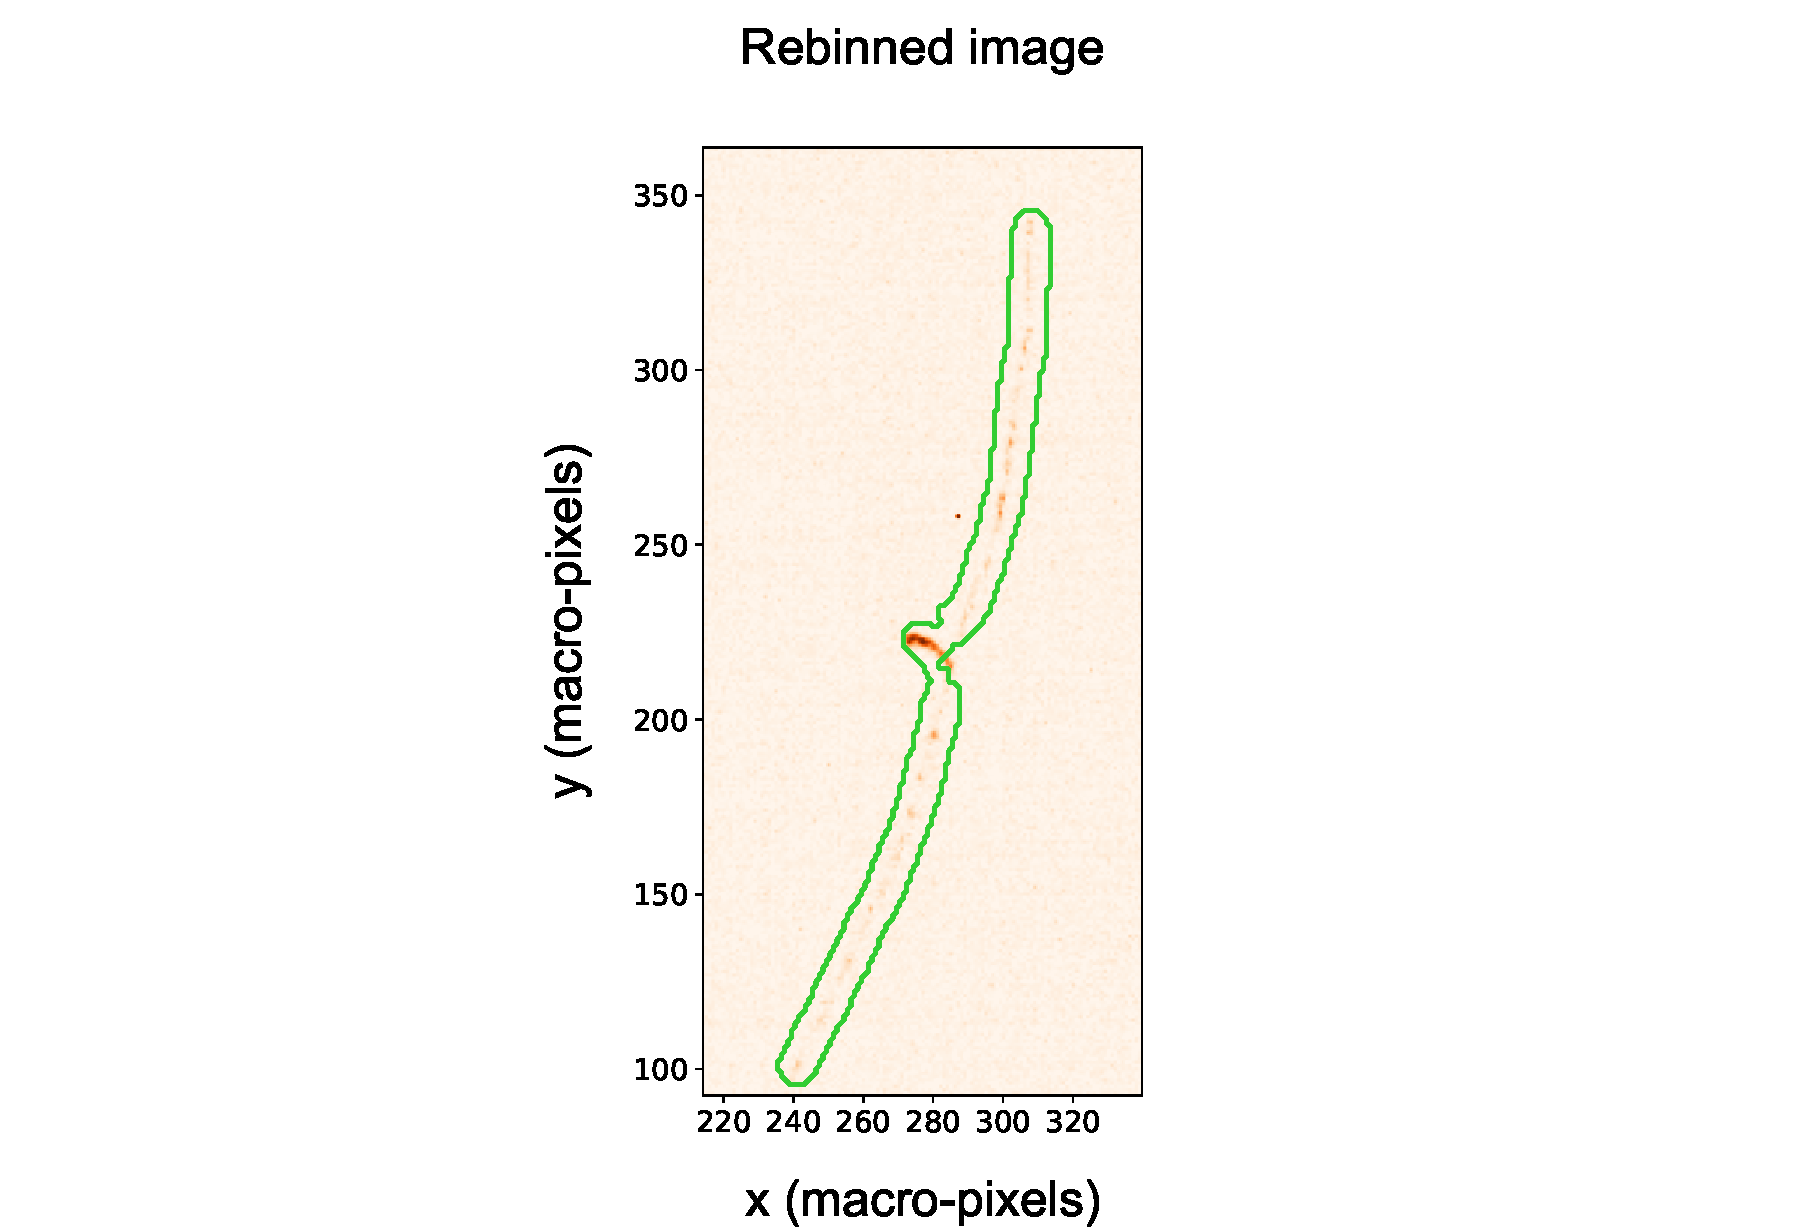
\includegraphics[width=0.49\linewidth]{figures/pic_run02156_ev49_sc_3D_paper}
     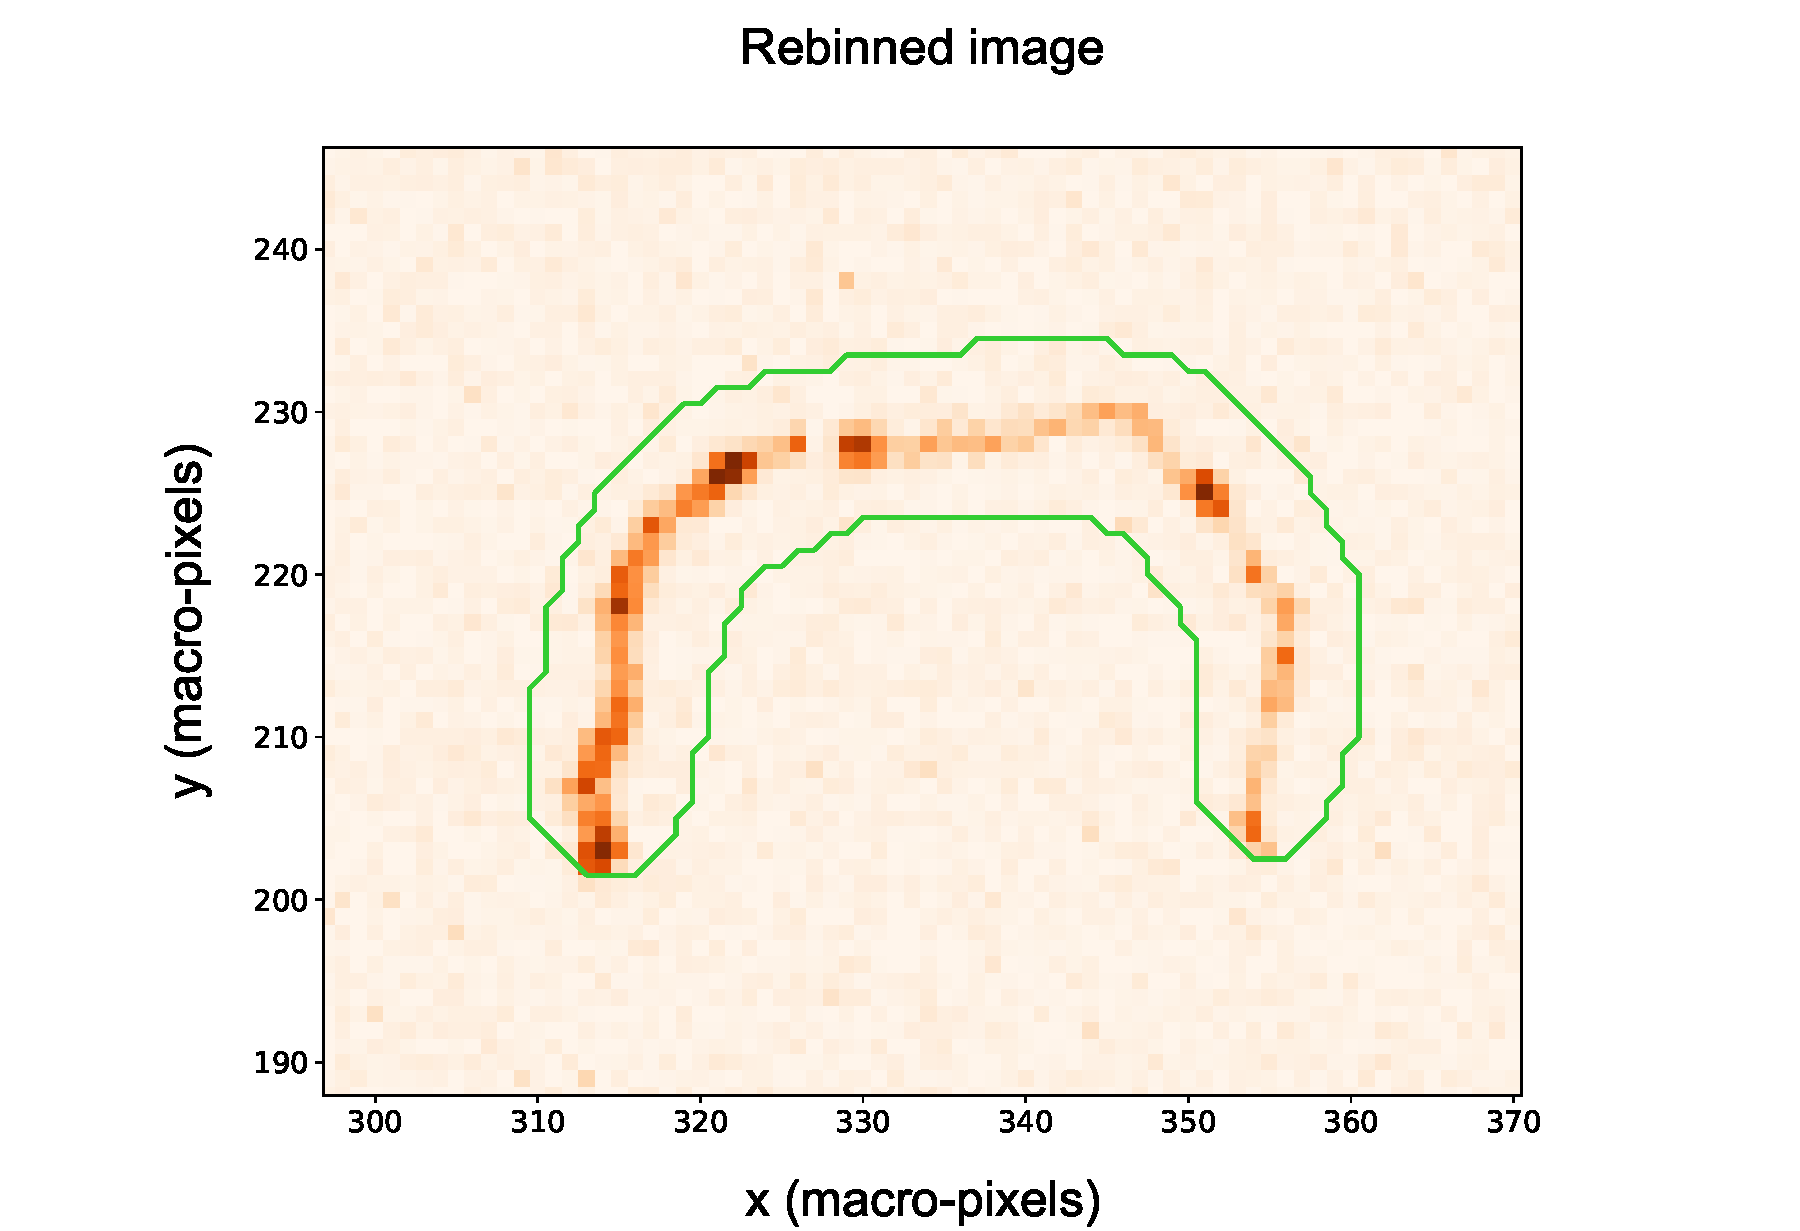
\includegraphics[width=0.49\linewidth]{figures/pic_run02156_ev641_sc_3D_paper} \\
     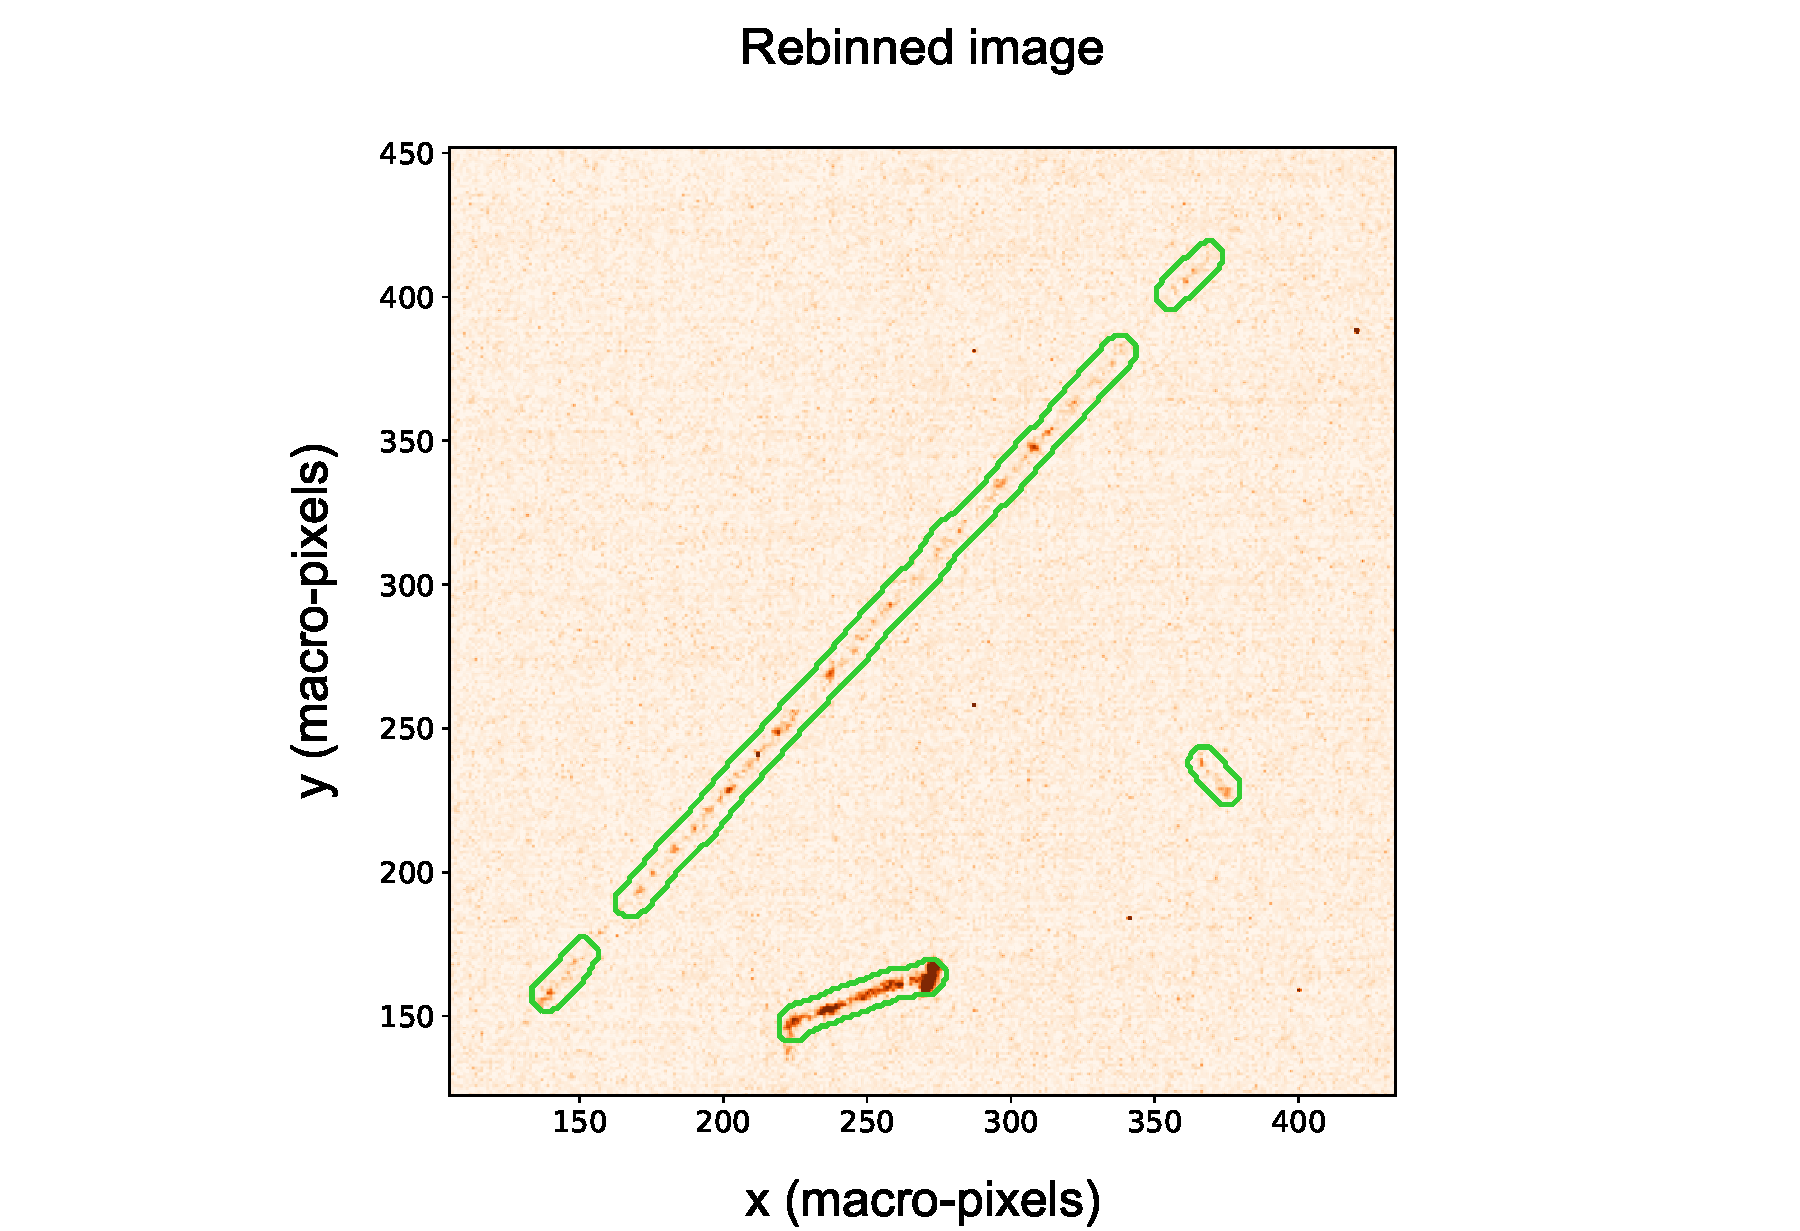
\includegraphics[width=0.6\linewidth]{figures/pic_run02156_ev631_sc_3D_paper}
     \caption{Superclusters reconstructed in a run without radioactive
       sources.  Top left: cosmic ray track fully reconstructed by the \gac
       superclustering. A $\delta$-ray is included in the supercluster. Top right: curly track from a candidate of
       natural radioactivity interaction. Bottom: a cosmic ray with the
       extremes not joined to the main track, plus a curly track from
       natural radioactivity. \label{fig:super_clusters2}}
  \end{center}
\end{figure}


\subsection{Super clusters calibration}
\label{sec:calibration}
The containment of the energy in the supercluster was verified
with simulations of nuclear and electron recoils  within
the gas mixture of the \lemon detector, performed with
\SRIM~\cite{bib:srim}.  For both types of recoils,
for the energy range of interest for DM search, \ie, $E \lesssim
100$\keV, when considering deposits without electronics noise and no
diffusion in the gas, the peak of the $\abs{E-E_{true}}/E_{true}$
distribution is within 5\%. Adding a noise approximated as a Gaussian
function with a mean and a SD equal to the ones observed in the
pedestal runs, and a diffusion following the parameterization in
Eq.~\ref{eq:diff}, the fraction of the true energy contained in the
supercluster decreases to about 80\%.
%
The decrease in the energy containment in the supercluster is due to
the smearing of the 2D track pattern around the periphery of the
cluster, mostly due to the diffusion effect.  This decreases the
gradients in Eq.~\ref{eq:gradient} around the edges, and so the
supercluster can shrink more around the crest, loosing part of the
tails that can be confused more easily with the noise.  A more
realistic noise description, and an improved diffusion model, based on
the one measured in data is necessary to tune the supercluster
parameters in simulation to recover part of the containment.  The
energy resolution found in simulation (around 4\%) is far from the
measured one in data, around 18\%, because of the absence, in the
simulation, of the dominant contribution of the response fluctuations:
Poissonian distribution of the number of primary electrons ionized in
the gas and exponential behavior of the number of secondary electrons
produced in each GEM amplification stage~\cite{bib:thesis}. Both of
them are expected to give rise to fluctuations of the order to 10\%,
that, once added in quadrature, can account for a large part of the
measured energy resolution.

The absolute energy scale was then calibrated with the energy
distribution measured in data with the \fe source, which provides
monochromatic photons of 5.9\keV, with the procedure described in
Ref.~\cite{bib:fe55}. The supercluster integral is defined as:
\begin{equation}
\label{eq:integral}
I_{SC} = \sum_i^{cluster} N_{ph}^i,
\end{equation}
where $N_{ph}^i$ is the number of counts (photons) in the $i^{th}$
pixel, and the sum runs over all the pixels of the supercluster.
While to perform the basic- and super-clustering only pixels passing
the zero suppression are considered, for the energy estimate in
Eq.~\ref{eq:integral} all the pixels within the cluster contours are
counted, eventually having negative $N_{ph}^i$ after the pedestal
subtraction. This choice is meant to avoid a bias on the energy
estimate, since after the pedestal subtraction the distribution of the
noise is centered around zero.  The distribution of \isclu, for a run
taken in presence of \fe source, is shown in
Fig.~\ref{fig:feuncalibpeak}. In addition to the main peak, with a
mean of about 2500\unit{counts}, a broader peak is clearly
distinguished, which represents the cases of two merged spots, with an
integral twice the single spot one. An example of such a merged spot
is given in Fig.~\ref{fig:basic_clusters} (left).
%
\begin{figure}[ht]
  \begin{center}
    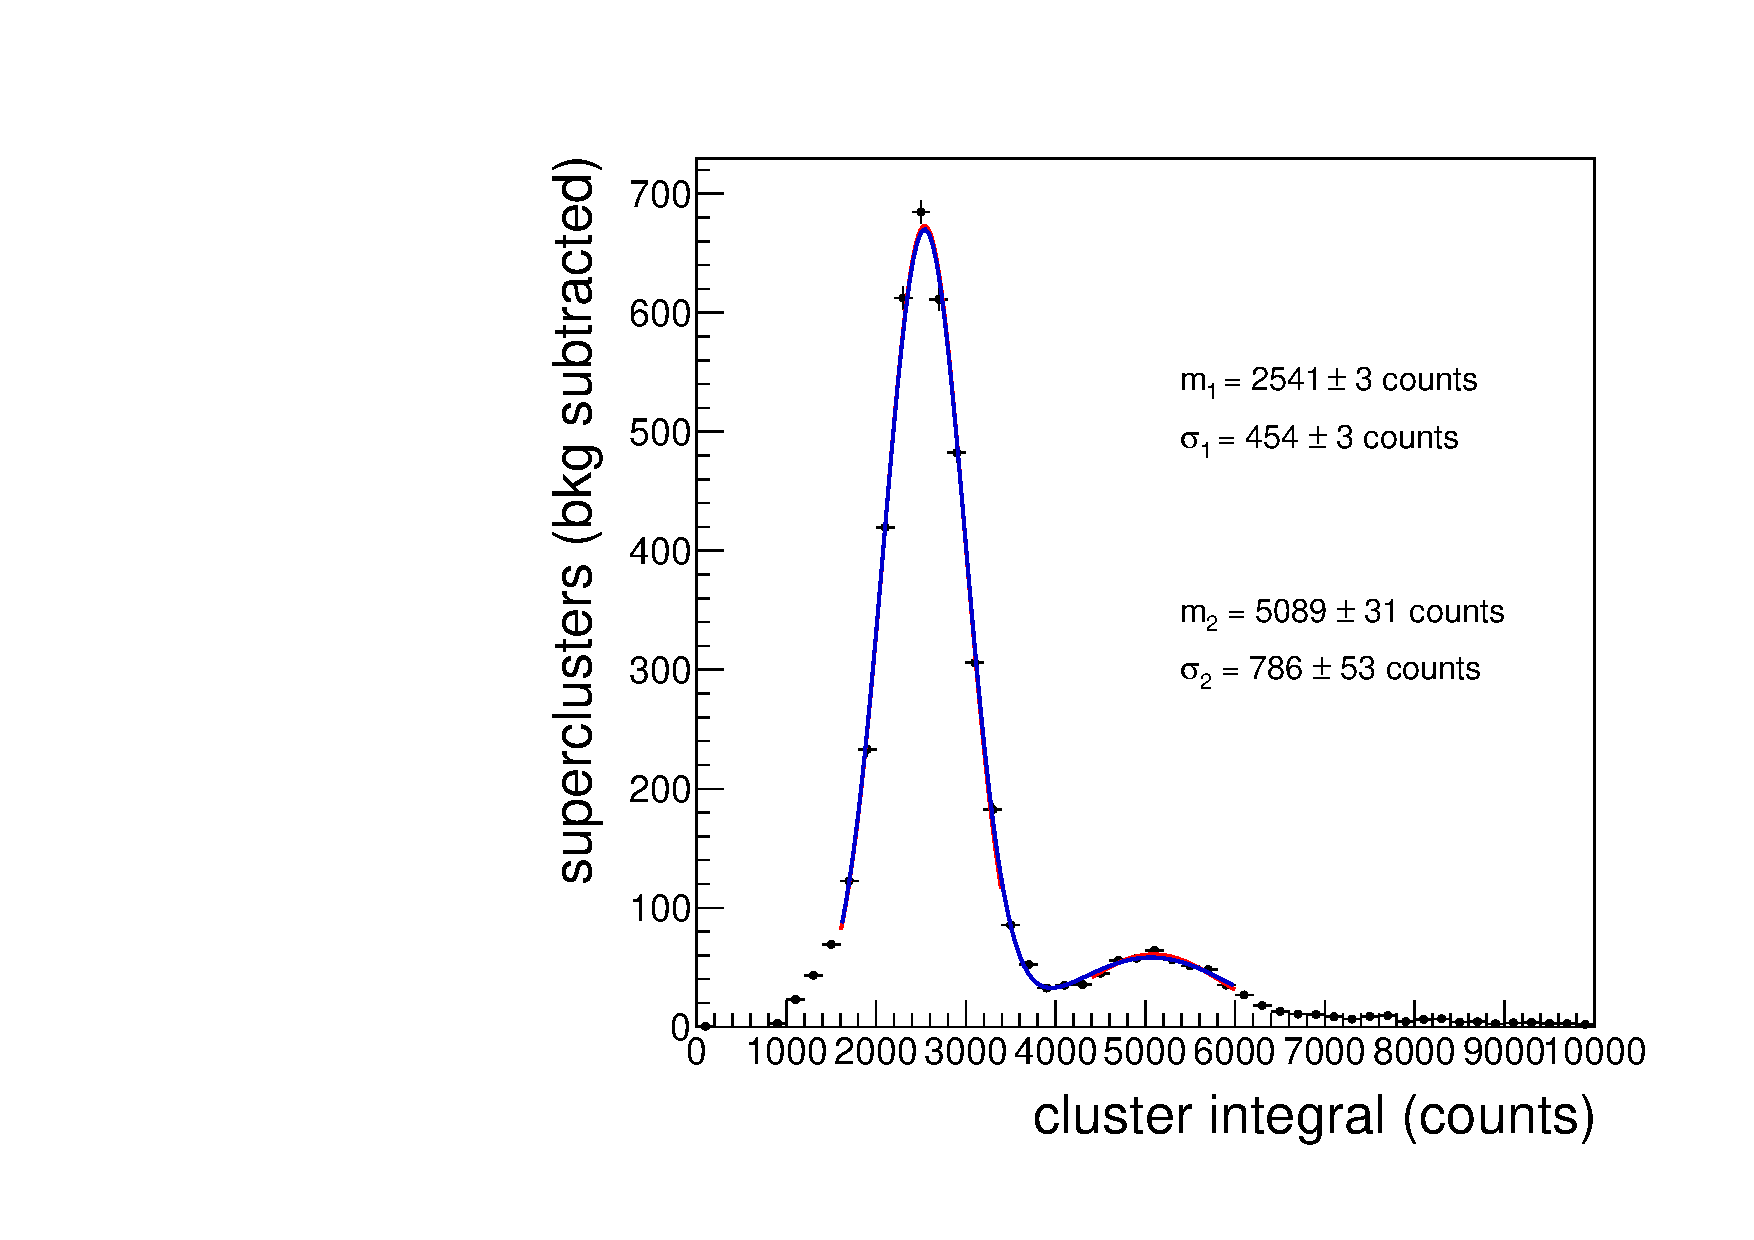
\includegraphics[width=0.49\linewidth]{figures/fe_ucalibintegral_fit}
    \caption{Distribution of the supercluster integral, before the
      absolute energy scale calibration is applied, in events with the
      \fe source. Clearly visible is the large peak of a single spot,
      and, at around twice the energy, a broader peak for the case of
      two neighboring spots merged in a single supercluster.
      \label{fig:feuncalibpeak}}
  \end{center}
\end{figure}
%
 The position of the maximum in the single-spot distribution in runs
with \fe source allowed to calibrate the absolute energy scale of
the \lemon detector.  The energy resolution for the reconstructed \gac
superclusters is about 18\%, similar to the one that can be obtained
with only the basic clustering step with \idbscan~\cite{iDBSCAN}, and
improving the one with the simple \nnc algorithm previously
used~\cite{bib:fe55}.

Using runs with this monochromatic, high rate source, positioned at
different distances from the GEM planes, a decrease of the light
response for lower distances from the GEM was observed. This effect is
opposite to the expected behavior of a lower light yield at larger
distances. Indeed, it is expected that, during the drift along the
$z$-direction, the ionization charge undergoes a diffusion in the TPC
gas, and some electrons are removed by attachment to the gas molecule.
Consequently, some loss in the light collection may be expected. The
opposite behavior, instead, is clearly observed. While this effect is
currently under study in more detail, it was attributed to a possible
saturation effect of the GEMs, especially in the third stage of
multiplication, where the charge density in one GEM hole is
maximal.  Under this hypothesis, an effective, empirical correction
was developed, which relies on the charge density of a cluster from
a \fe deposit. The light density, $\delta$, is defined as:
\begin{equation}
  \label{eq:density}
  \delta = \isclu / n_p,
\end{equation}
where $n_p$ is the number of pixels passing the zero-suppression
threshold (differently from the definition of \isclu, where all the
pixels in the supercluster are considered). This effective calibration
returns the absolute energy of a spot-like region, similar in size to
the \fe clusters, as a function of the supercluster density, $\delta$:
$E=c(\delta)\cdot I_{SC}$. In the hypothesis of saturation, the
\textit{local} density along the track is the parameter which
regulates the magnitude of the effect, thus the correction has to be
applied dynamically for slices of the supercluster having a size
similar to the \fe spots.  This is achieved with the procedure
described in the following.

First, the supercluster \textit{skeleton}, \ie, the 1-pixel-wide
representation along the path, is reconstructed.  This is achieved
through a morphological thinning of the superclusters with the iterative
algorithm from Ref.~\cite{thin1,thin2}.  Second, a pruning of the
obtained skeleton is done, to remove residual small branches along the
main pattern, using a hit-or-miss transform. The output of this
process for one example track is shown in Fig.~\ref{fig:skeleton}.
%
\begin{figure}[ht]
  \begin{center}
     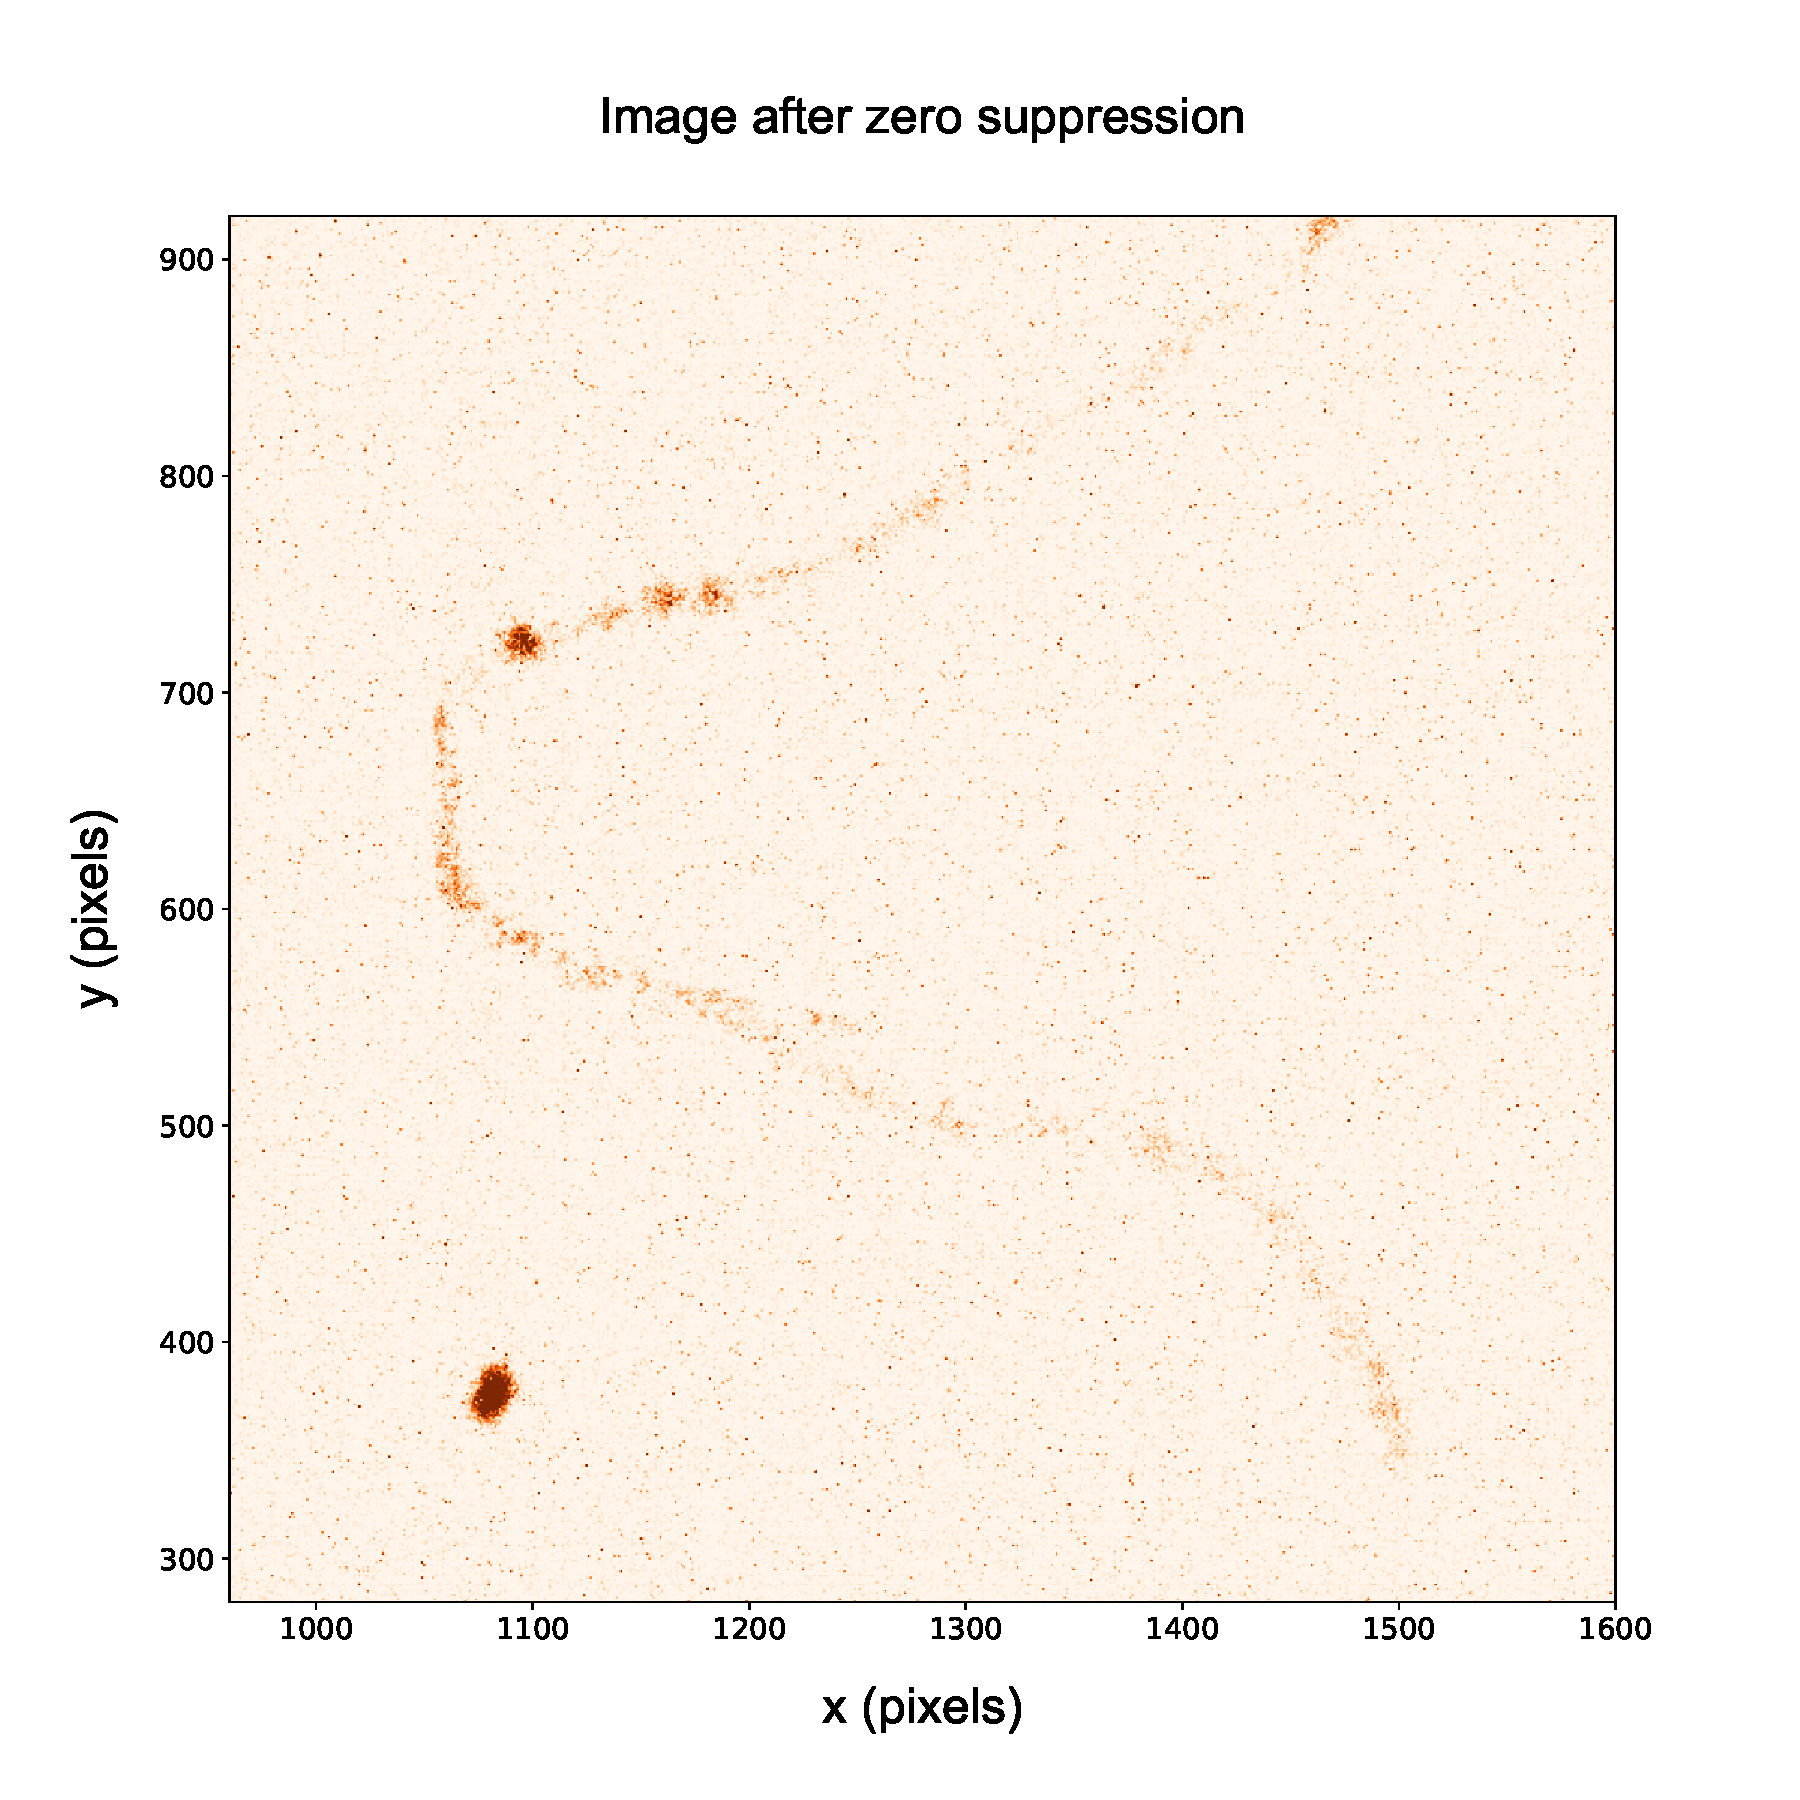
\includegraphics[width=0.49\linewidth]{figures/pic_run02317_ev8_oriIma_paper_zoom}
     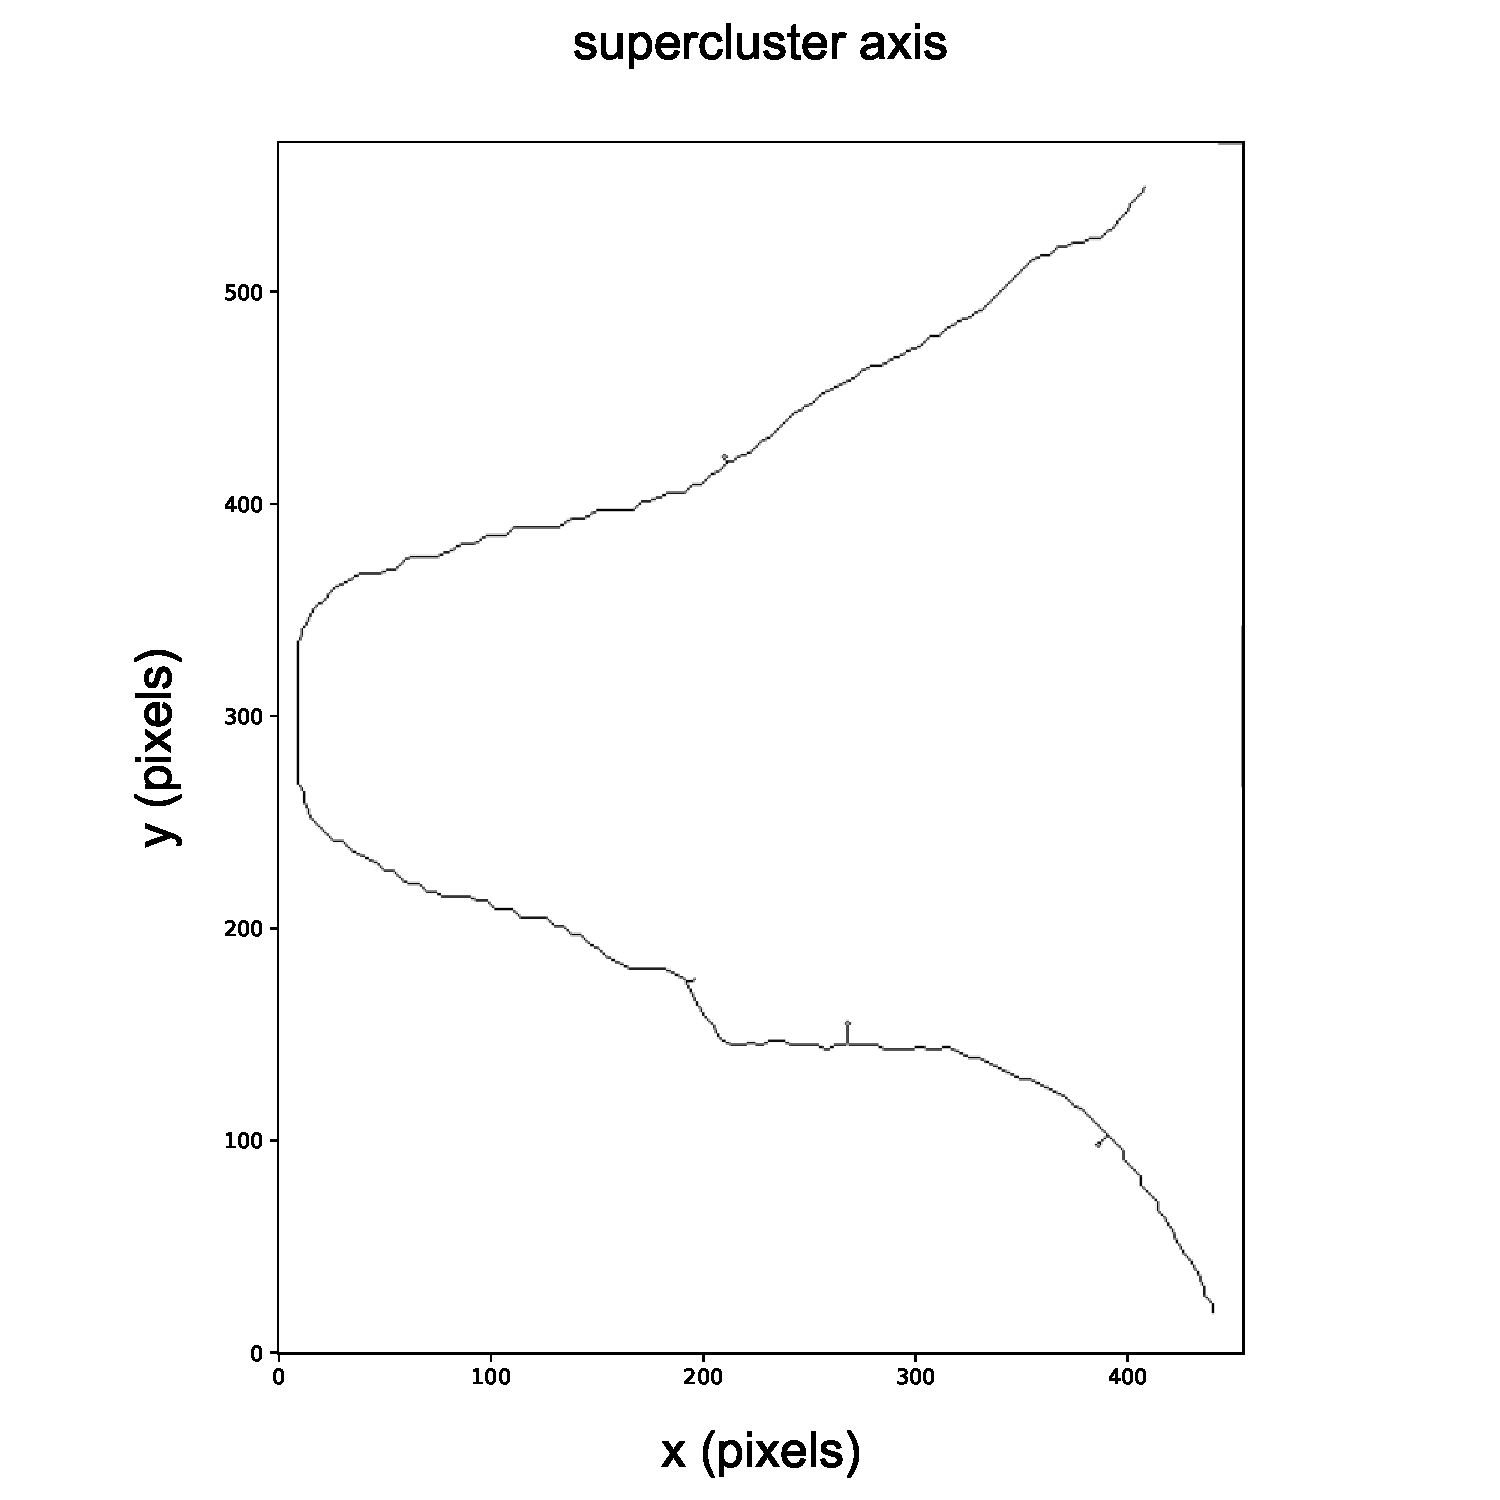
\includegraphics[width=0.49\linewidth]{figures/skeleton_paper}

      \caption{Left: zoom on the full-resolution image of a track
        candidate in a run with the \ambe radioactive source. Right:
        output of the skeletonization and pruning of the branches for
        one example supercluster extended in
        space.  \label{fig:skeleton}}

    \end{center}
\end{figure}
%
For the calibration procedure, the found skeleton is followed,
starting from one of the two end points, and circles having their
center on a pixel of the skeleton and their radius equal to the
average spot size of the \fe clusters are defined. It was checked
that this procedure includes all the pixels of the original cluster
for the vast majority of the clusters considered.  The local density
$\delta_s$ of the slice $s$ is computed, and its integral $I_s$ is
calibrated to an absolute energy through the effective correction
$E_s=c(\delta_s)\cdot I_s$. The pixels of the supercluster used for
the slice calibration are removed (including the skeleton ones), and
the procedure is iterated, until having included all the pixels. The
sum of the energies of all the slices is the estimate of the
calibrated energy of the supercluster:
%
\begin{equation}
  \label{eq:ecal}
  E_{SC} = \sum_s^{slices} E_s
\end{equation}
%
As a closure test of this procedure, the calibrated energy of the
superclusters reconstructed in the runs with the \fe source is
obtained.  The value of the energy peak was obtained by fitting the
distribution with the same function used in
Fig.~\ref{fig:feuncalibpeak}, and equals to  $m_1 = 5.93 \pm 0.01$\keV,
compatible with the expected value. The calibration procedure is an
overkill for the case of the small \fe spots, but it is necessary for
very long cosmic ray tracks or even for medium-length superclusters
from nuclear and electron recoils.  The energy resolution worsen after
the calibration ($\sigma_1 = 1.48 \pm 0.01$, \ie, 25\% energy
resolution), as a sign that the empiric correction is still
suboptimal.

The skeletonization procedure provides a general method to estimate
the track length ($l_p$), accurate both in the case of straight and
curving track. As a check, it has been verified that, in the case of
straight tracks, the length extracted in this way coincides with the
length of the major axis estimated with a singular value decomposition
(SVD), described in the following section. For exactly round spots,
the skeleton would collapse in the center of the cluster and the
resulting length would be 1 pixel, but this completely symmetric case
never happens in the considered samples.



\section{Cluster observables}
\label{sec:clustershapes}
 
 Define  (projected) length $l$, light $L$, energy $E$ (light after calibration), density of light $\delta$ (and then $\frac{dE}{dl}$ after calibration but projected that's why I am using $dl$ !), slimness $S$
 
 Describe here briefly the $E$ calibration ? saturation effect removal ? 
 
\section{Nuclear recoil identification results}
 
 During the data-taking xxx frames were recorded in absence of any external source ({\it no-source} sample). In these frames the interaction of ultra-relativistic cosmic ray particles (mostly muons) are clearly visible  as  very long cluster. Internal radioactivity of the \lemon materials  also contribute several smaller size cluster.  It is then possible to define a pure sample of cosmic ray tracks by requiring $L$ > 13 cm and $S$ < 0.1  \textcolor{red}{che altro manca? }. The cosmic ray cluster identified with this selection show small values of  $\delta$ $\sim $ 5 well compatible with the small specific ionization of ultra-relativistic particles. 
 In Fig.\ref{fig:cosmics} we show the distribution of the observed $\frac{dE}{dl}$ for the no-source sample and for the Am-Be samples. The broadening of the distribution is mainly due to the specific energy loss fluctuation in the gas mixture of the cosmic ray particles.   Its mean value corrected for the effect of the angular distribution of the cosmic rays is   xx keV/cm that is in good agreement with the Garfield prediction of 2.3 keV/cm.  The angle with the horizontal axis is evaluated by  measuring the distance between \textcolor{red}{EAM spiega come hai fatto}. In Fig.\ref{fig:cosmics} the distribution   of the  angle of the cosmic ray cluster in the no-source sample is shown.
 
 
 \begin{figure}[ht]
	\centering
	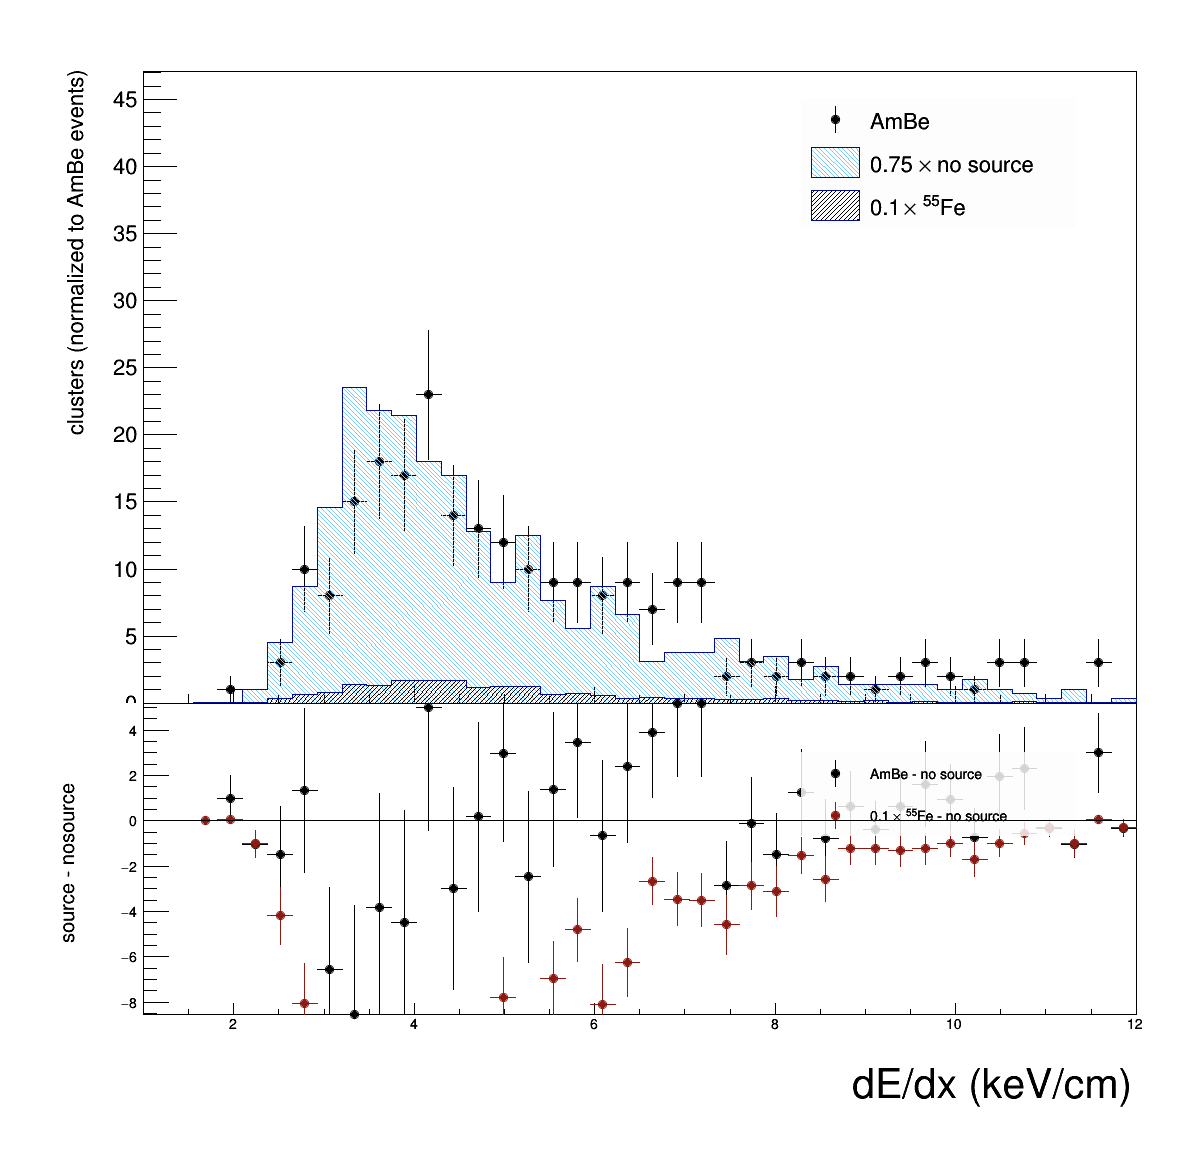
\includegraphics[width=0.45\linewidth]{dEdx_cosmics.png}
	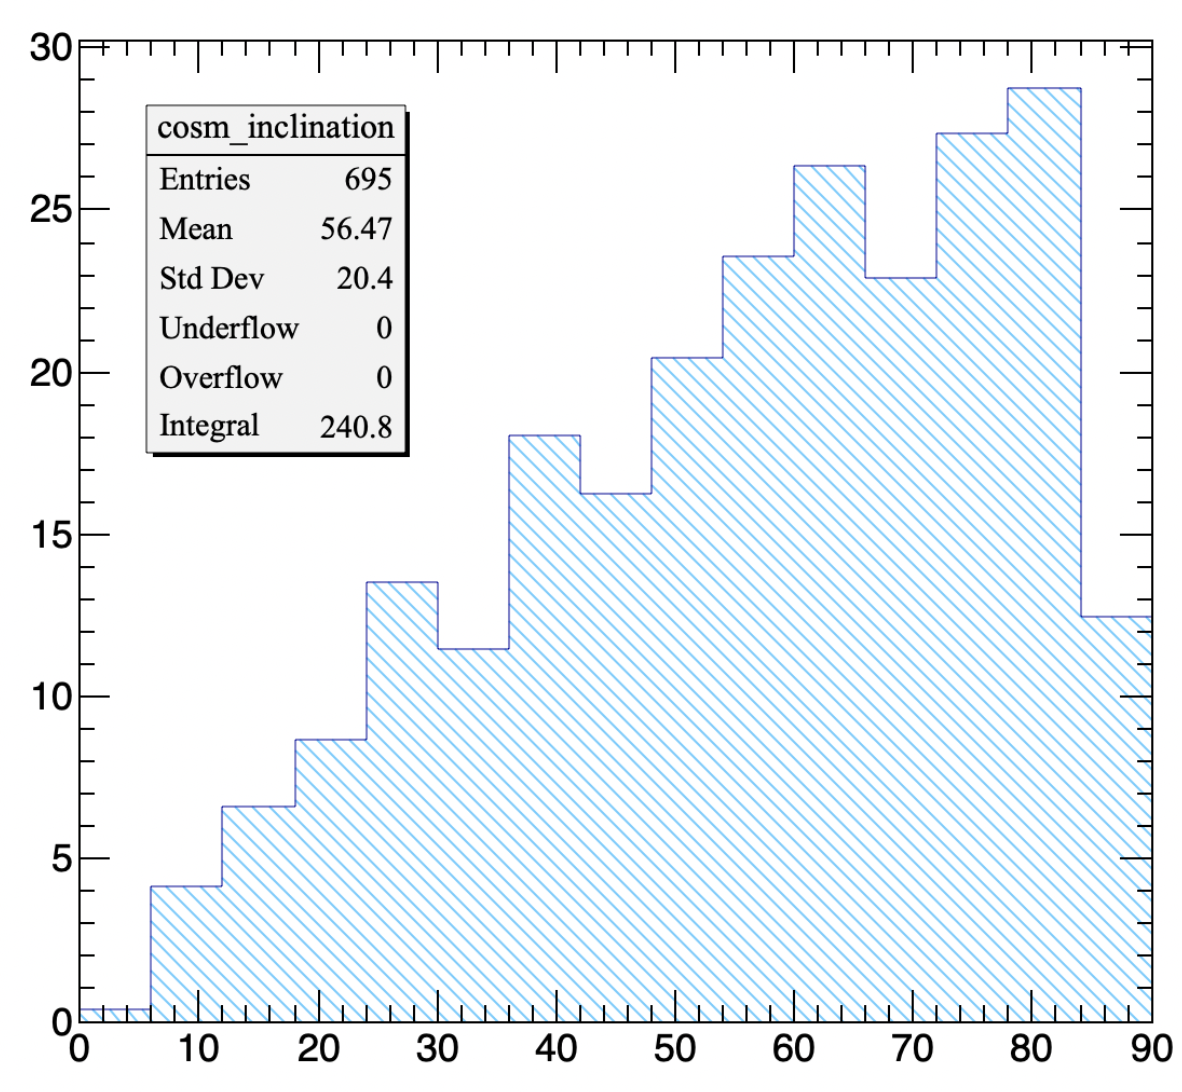
\includegraphics[width=0.45\linewidth]{cosmic_angle.png}
  	\caption{Left: Distributions of reconstructed energy release per centimetre for cosmic rays. Right: Distributions of reconstructed angles for cosmic rays. }
  	\label{fig:cosmics}
\end{figure}
\textcolor{red}{Non farei vedere il Ferro in questa figura. Inoltre il plot delle differenza deve essere fatto su scala diversa. }

 
 \section{Conclusion and Outlook}
 
 


\begin{figure}[ht]
	\centering
	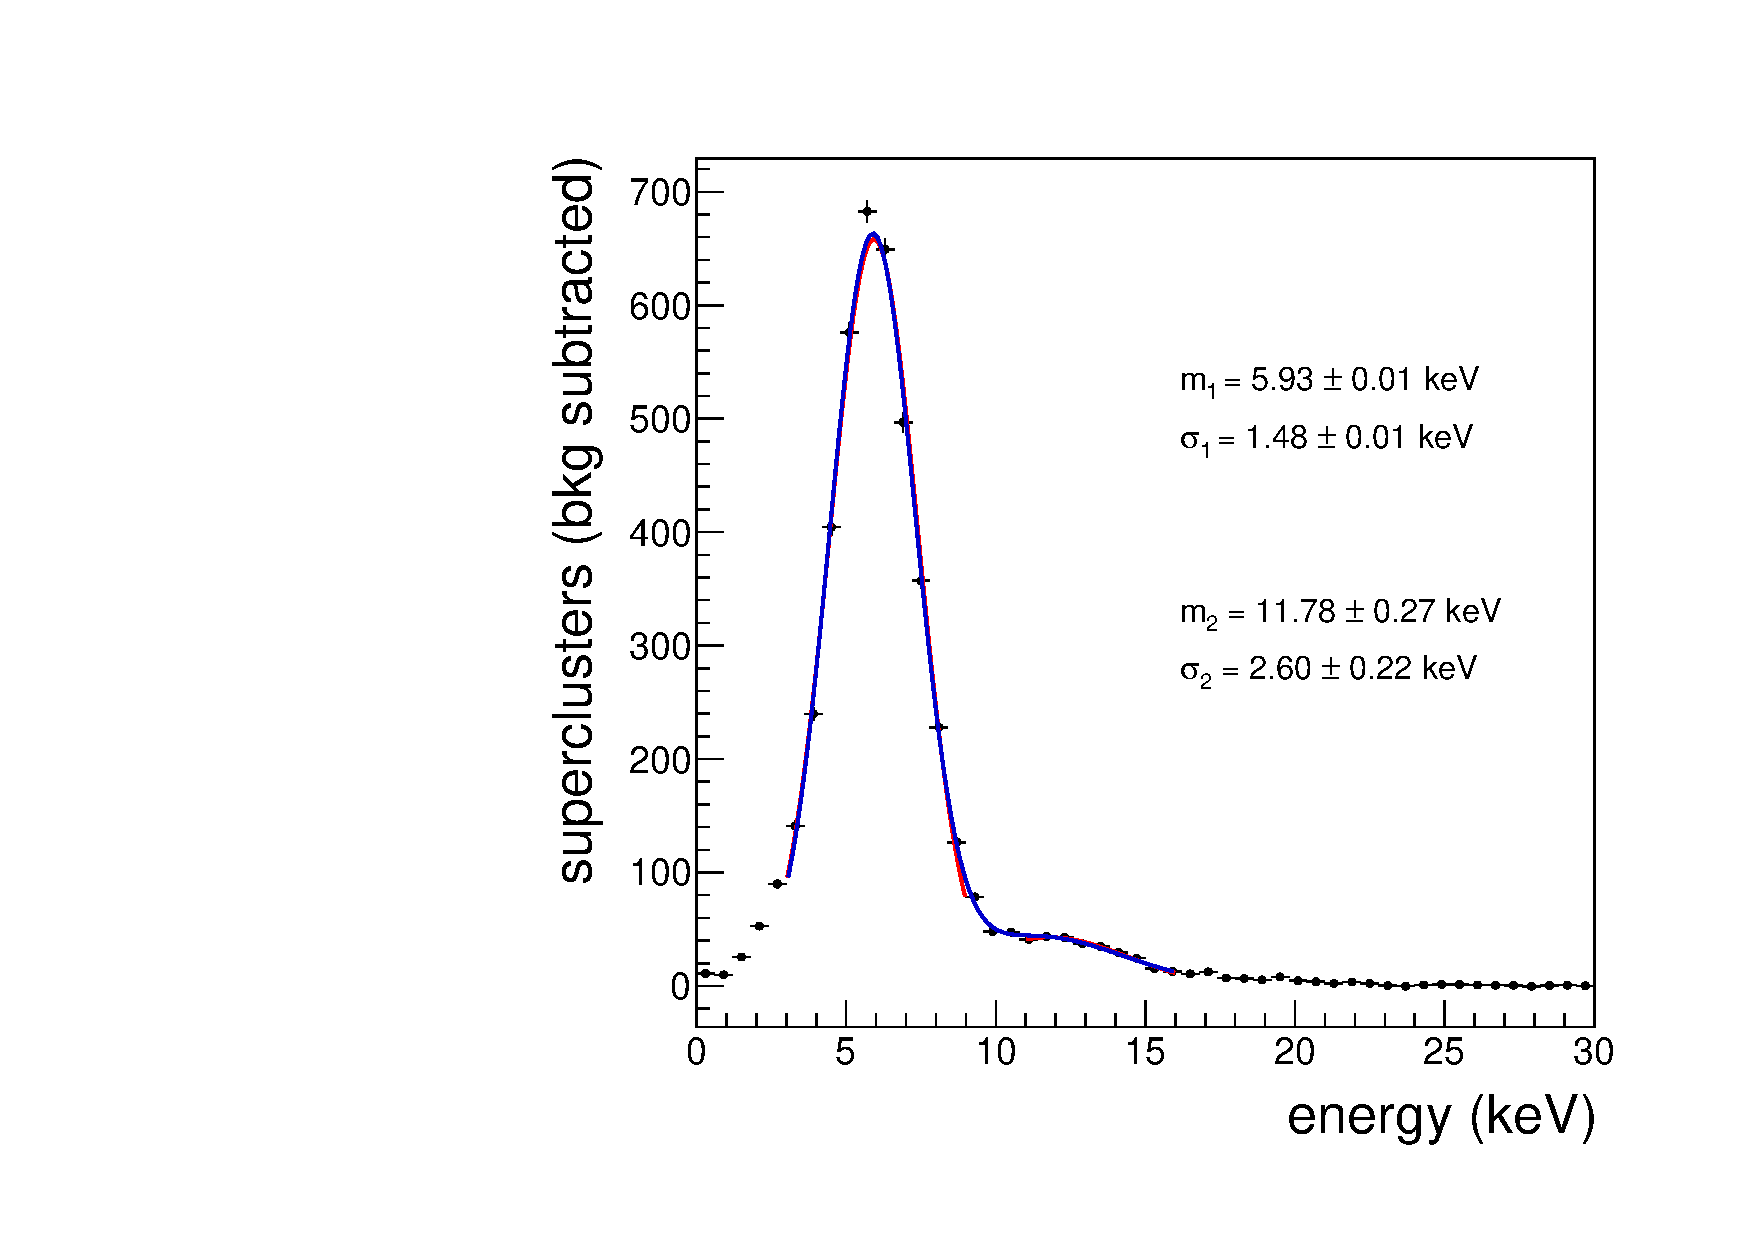
\includegraphics[width=0.45\linewidth]{fe_diff_simplefit.pdf}
	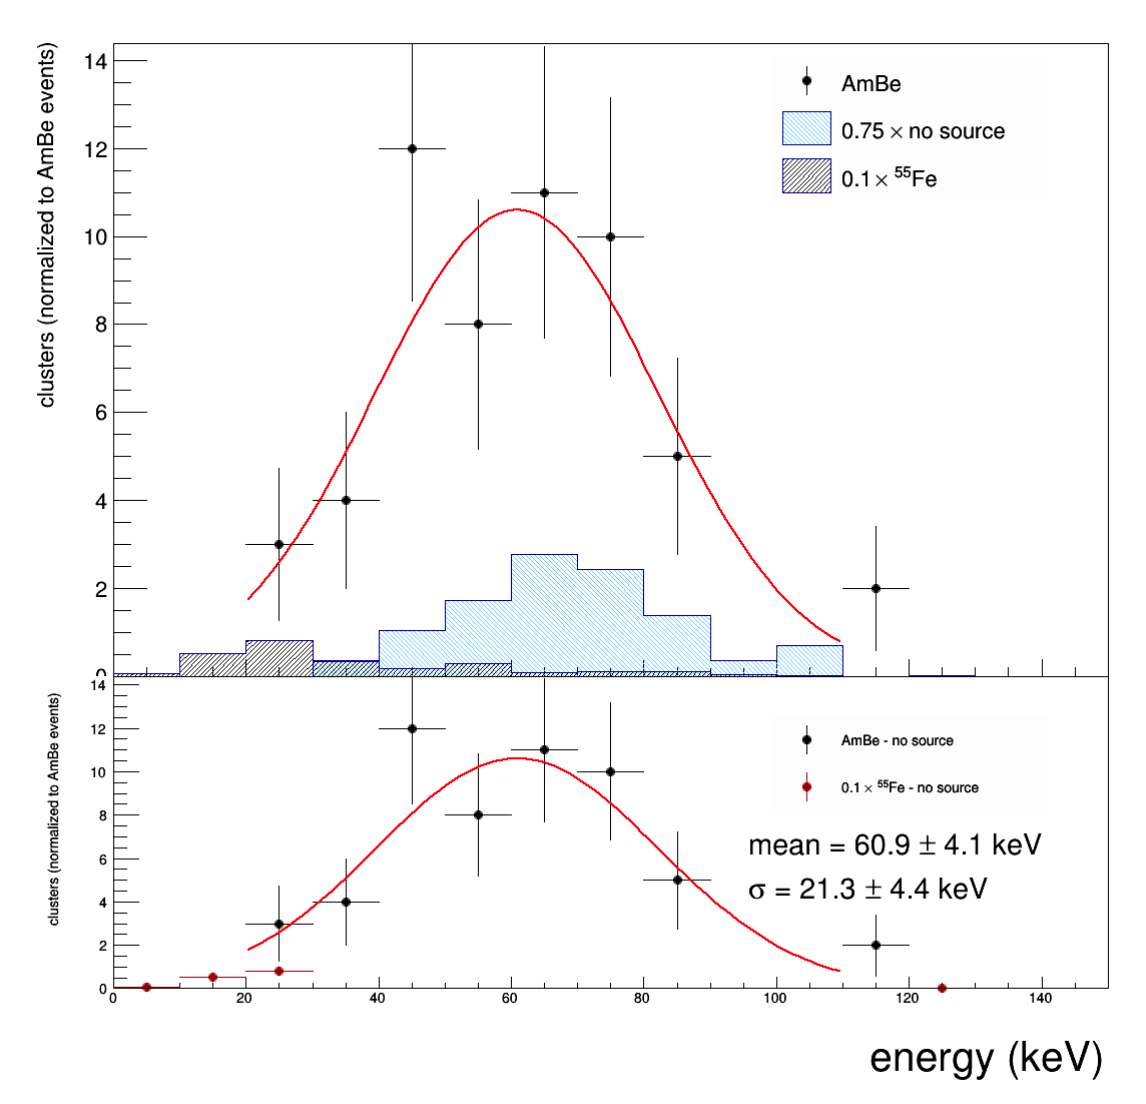
\includegraphics[width=0.45\linewidth]{spectrum_59keV.png}
  	\caption{Left: Spectrum of energy of the clusters reconstructed as produced by interactions of 5.9~keV photons in gas. Right: Spectrum of energy of the clusters reconstructed as produced by interactions of 59~keV photons in gas.}
  	\label{fig:55Fe&59keV}
\end{figure}

\begin{figure}[ht]
	\centering
	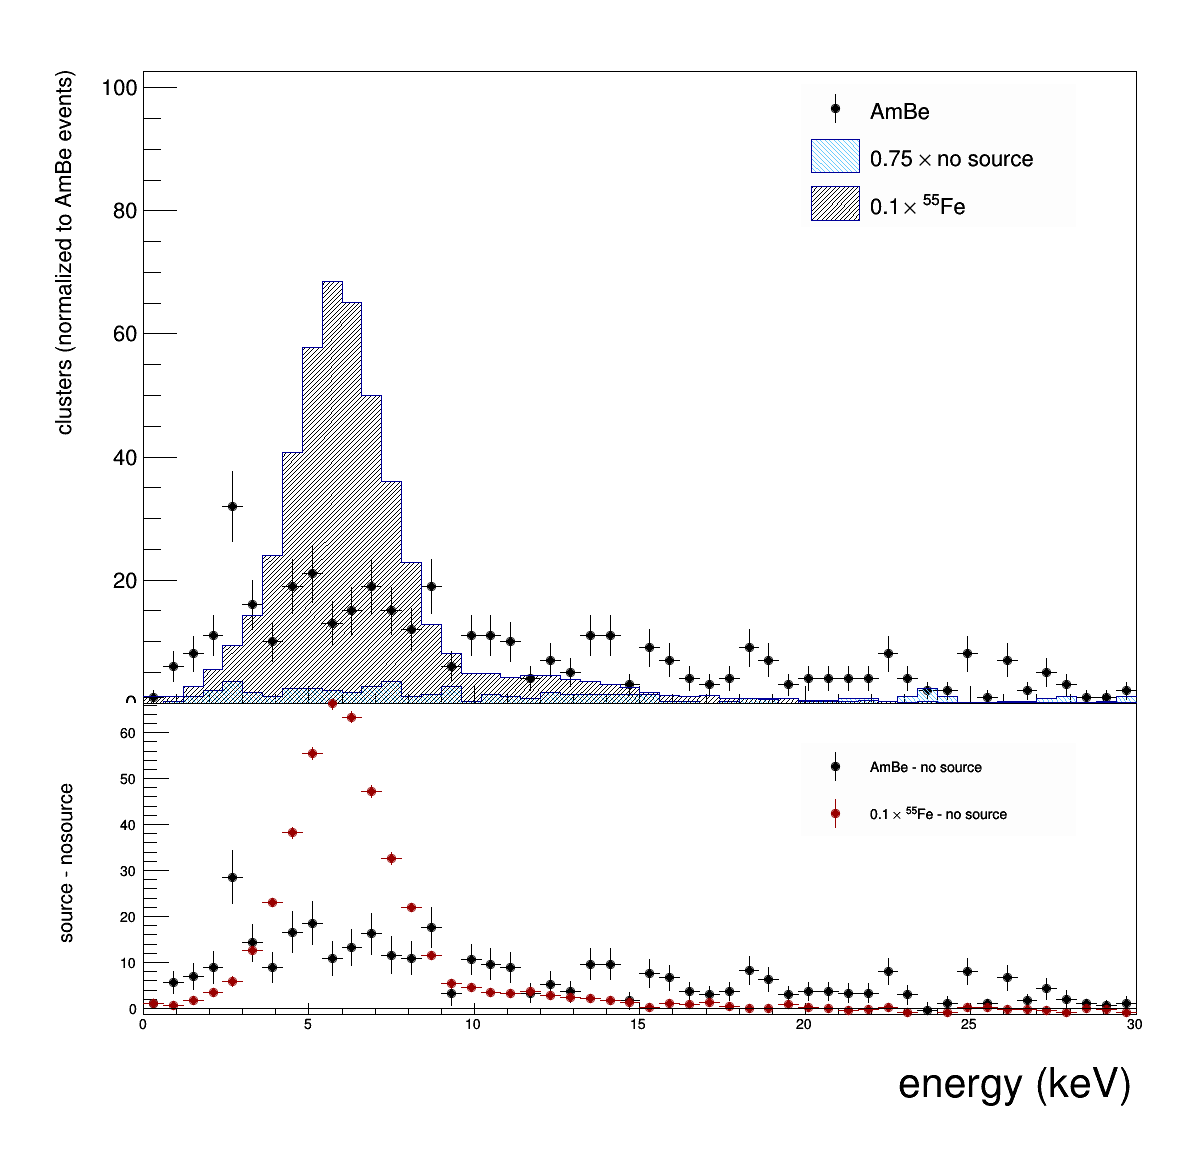
\includegraphics[width=0.45\linewidth]{energy_spectrum.png}
	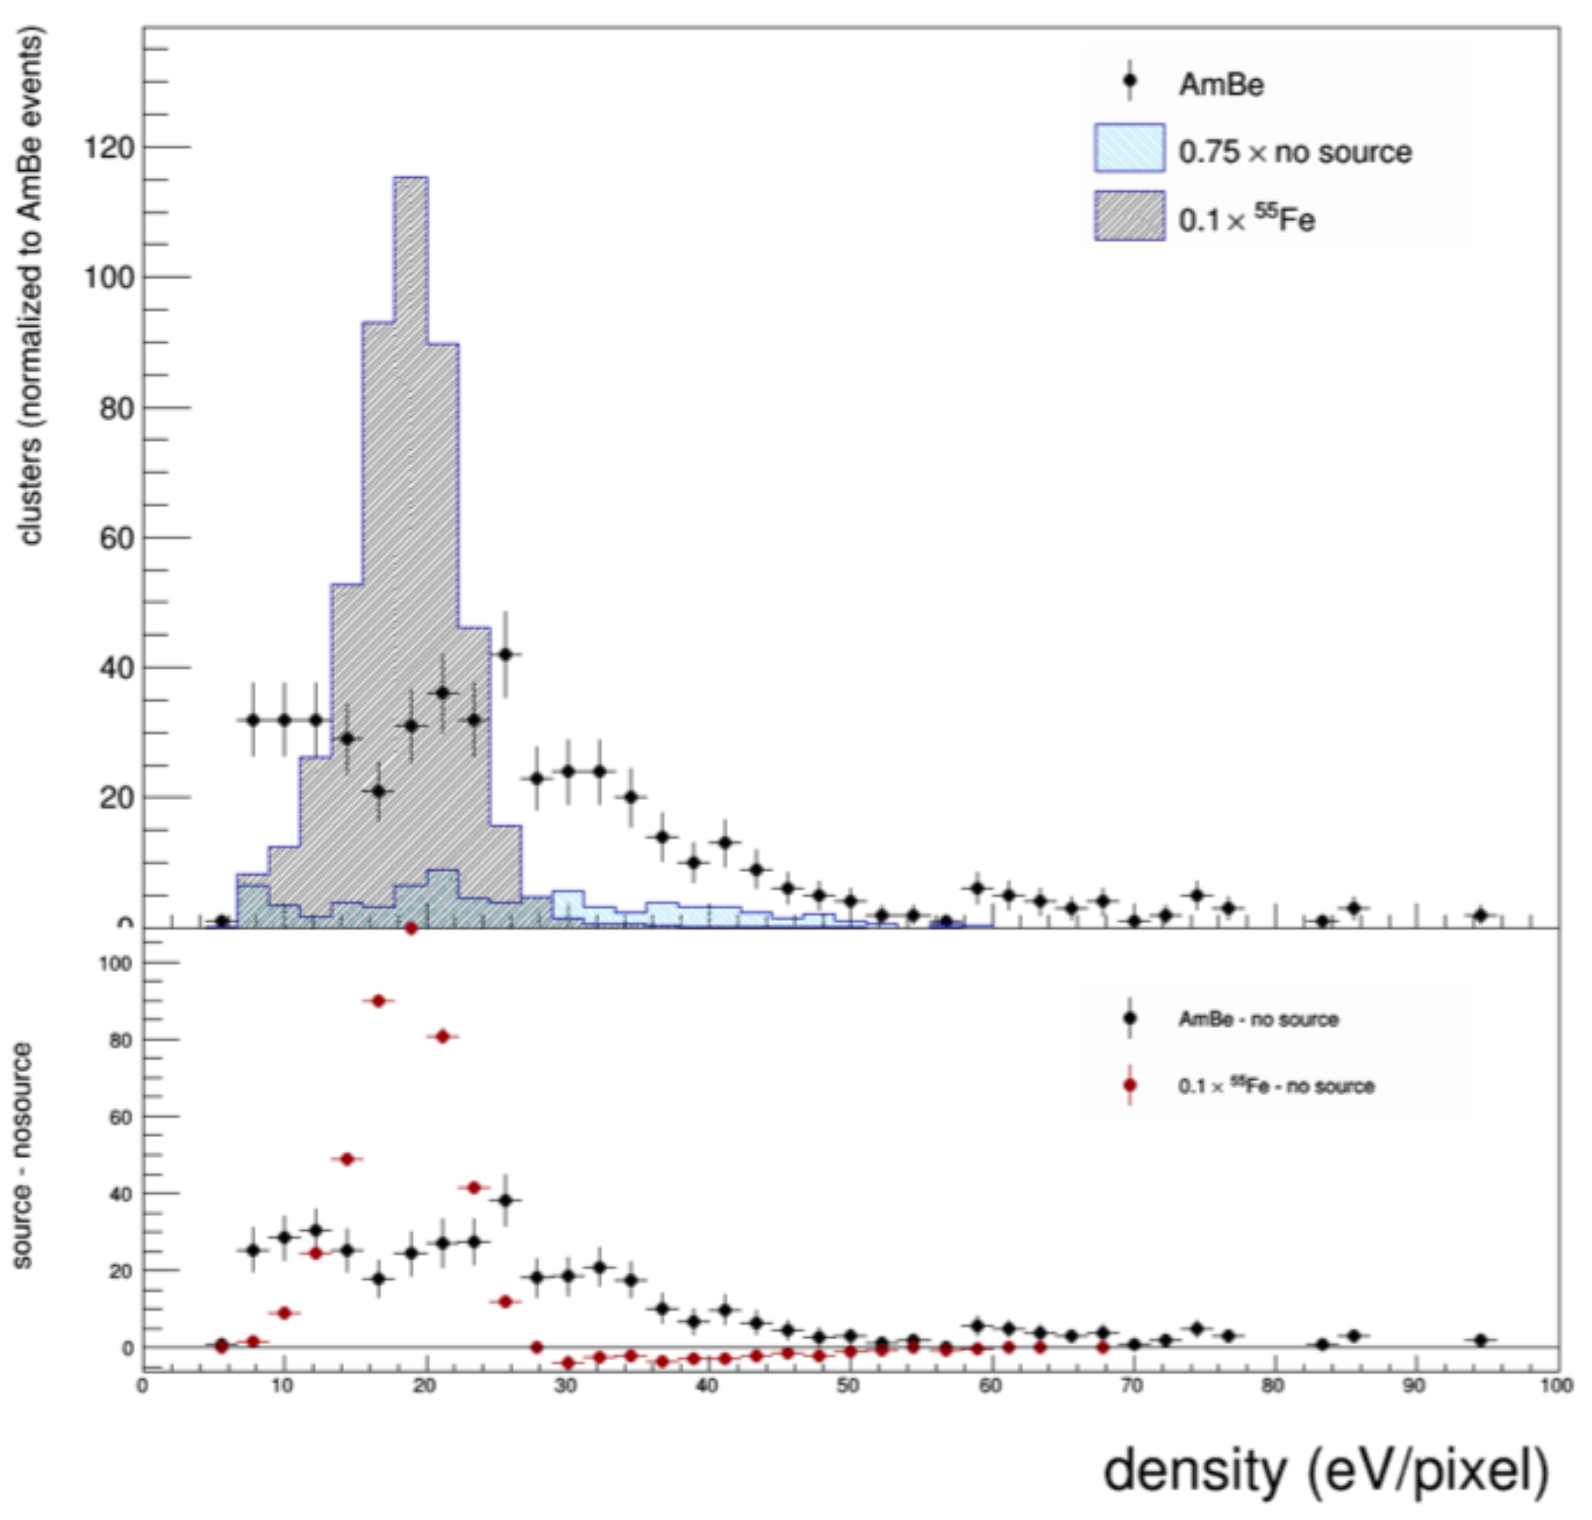
\includegraphics[width=0.45\linewidth]{density_spectrum.png}
  	\caption{Spectra of energy (left) and energy density (right) of the clusters reconstructed in three different run types after the preliminary cuts.}
  	\label{fig:ene&dens}
\end{figure}

\begin{figure}[ht]
	\centering
	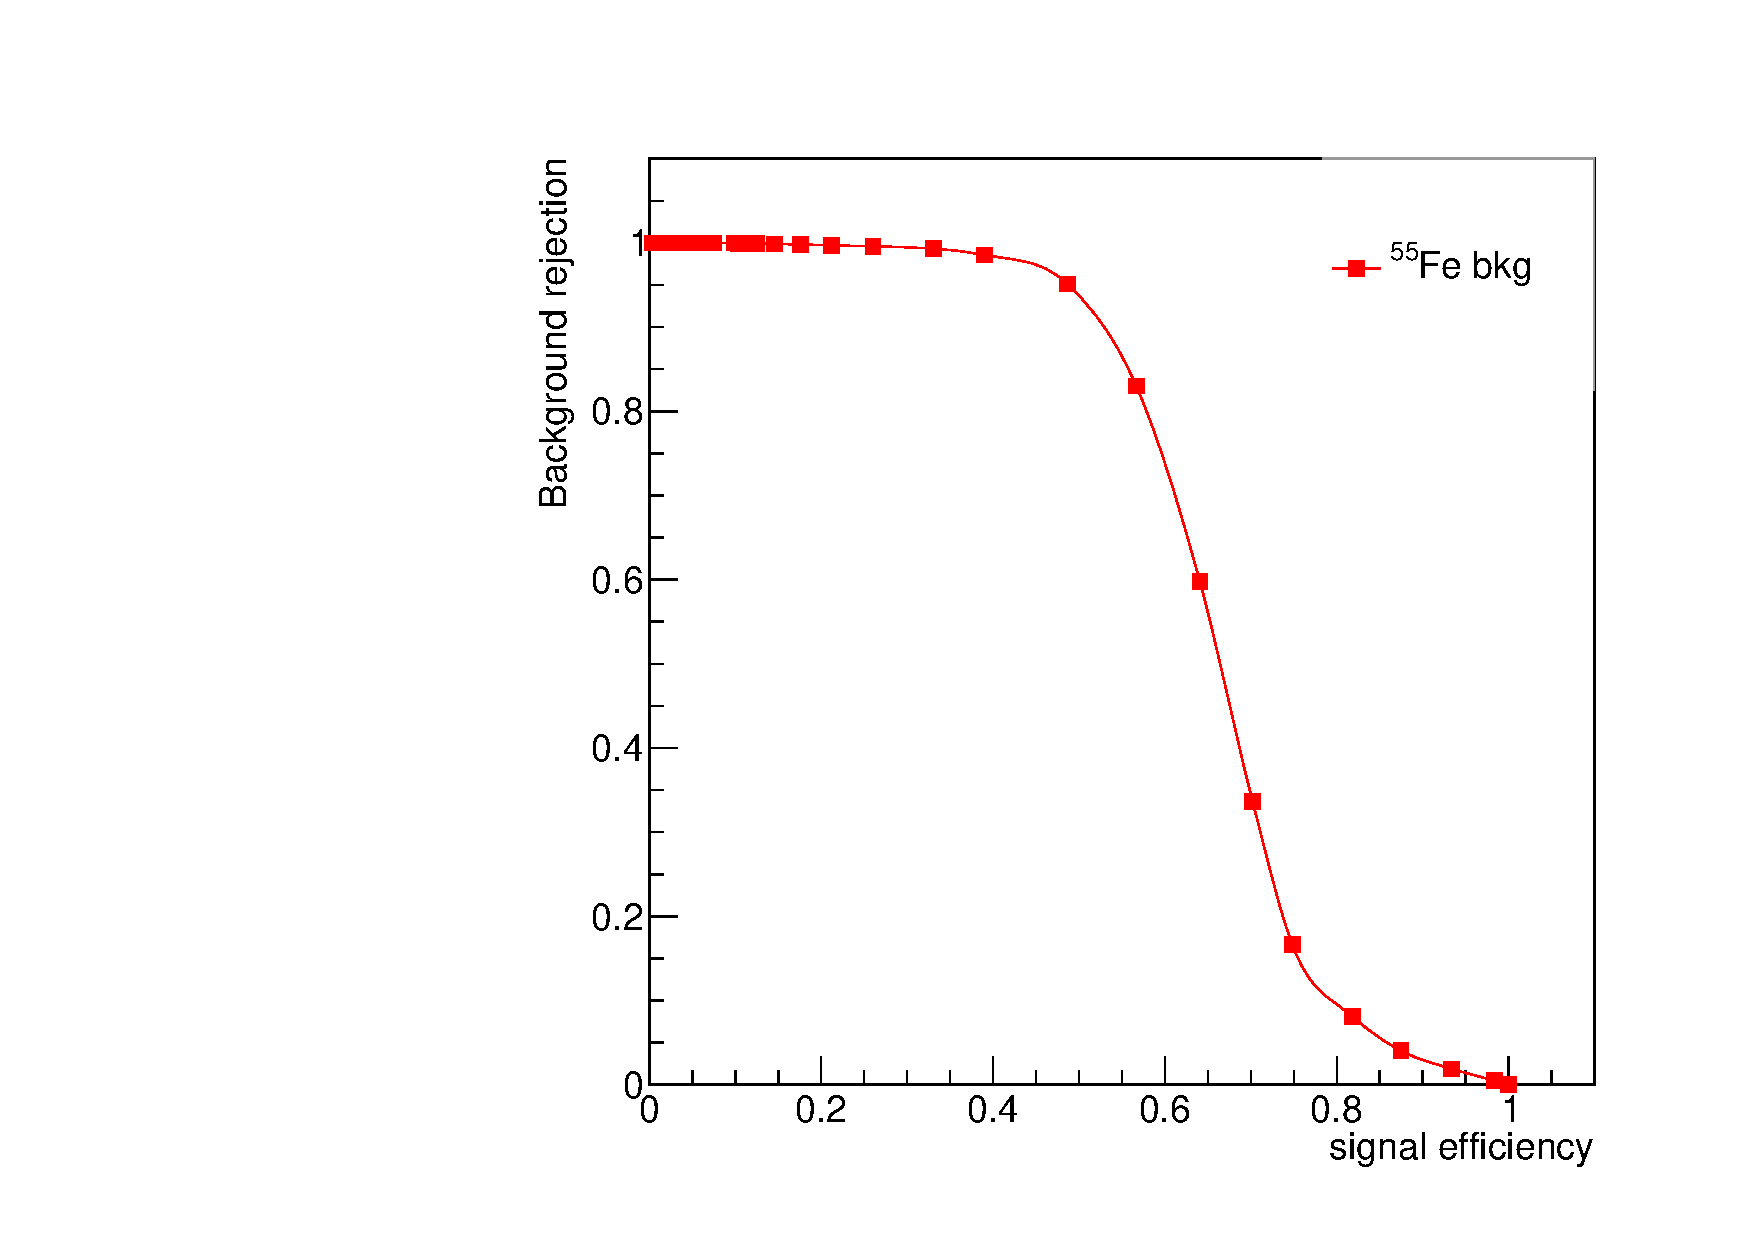
\includegraphics[width=0.50\linewidth]{density_roc.pdf}
  	\caption{Electron Recoil (ER) signal rejection as a function of the Nuclear Recoil signal detection efficiency.}
  	\label{fig:roc}
\end{figure}
\textcolor{red}{per un paio di punti scriverei vicino il taglio density > ...}

\begin{figure}[ht]
	\centering
	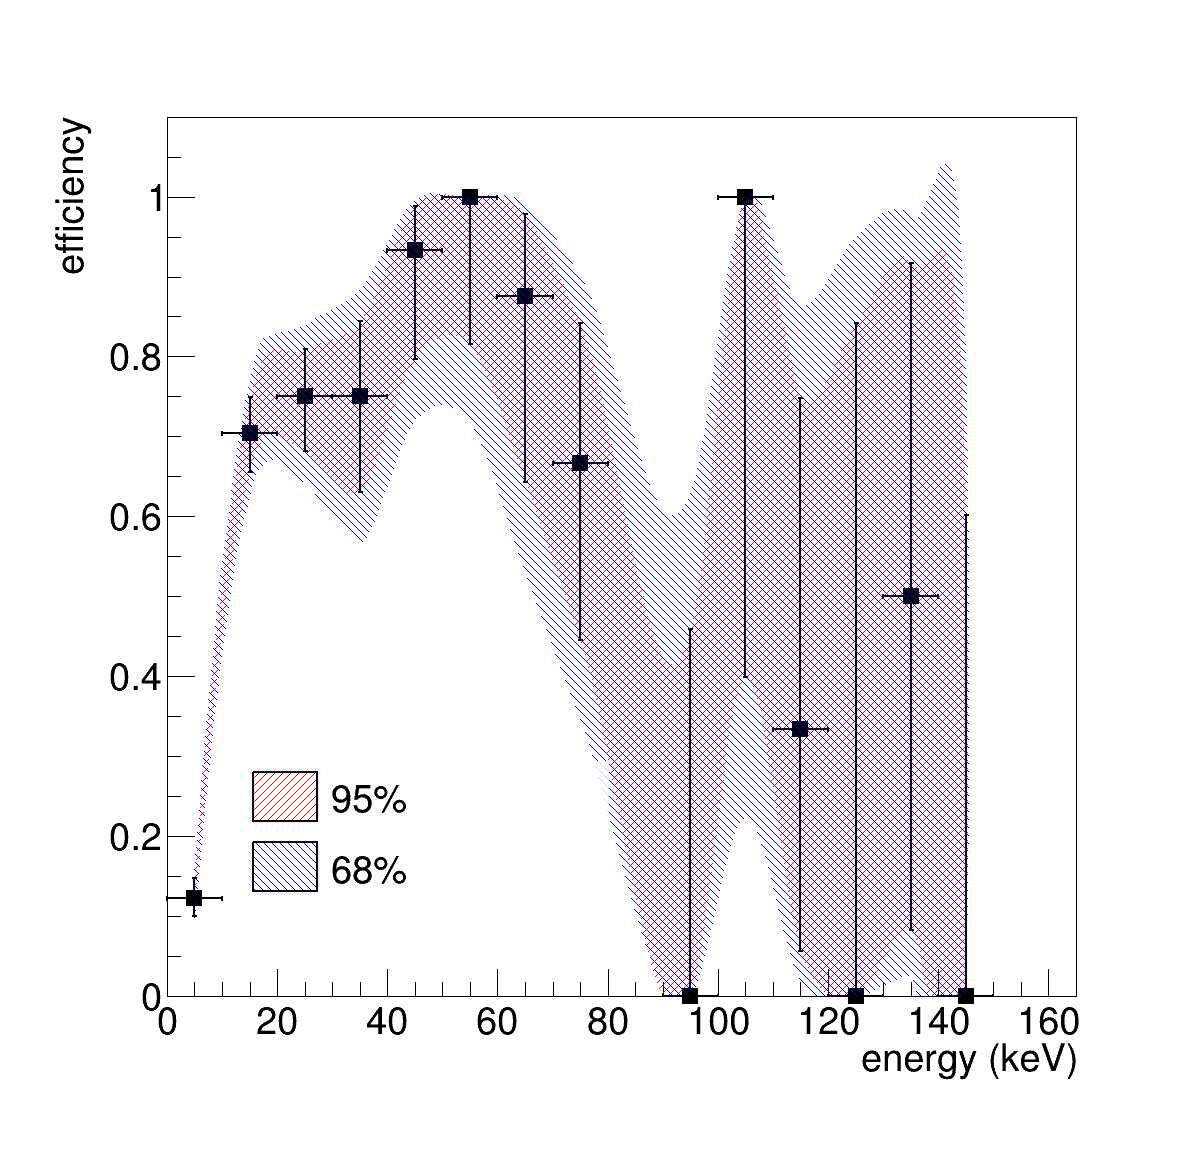
\includegraphics[width=0.45\linewidth]{effS.png}	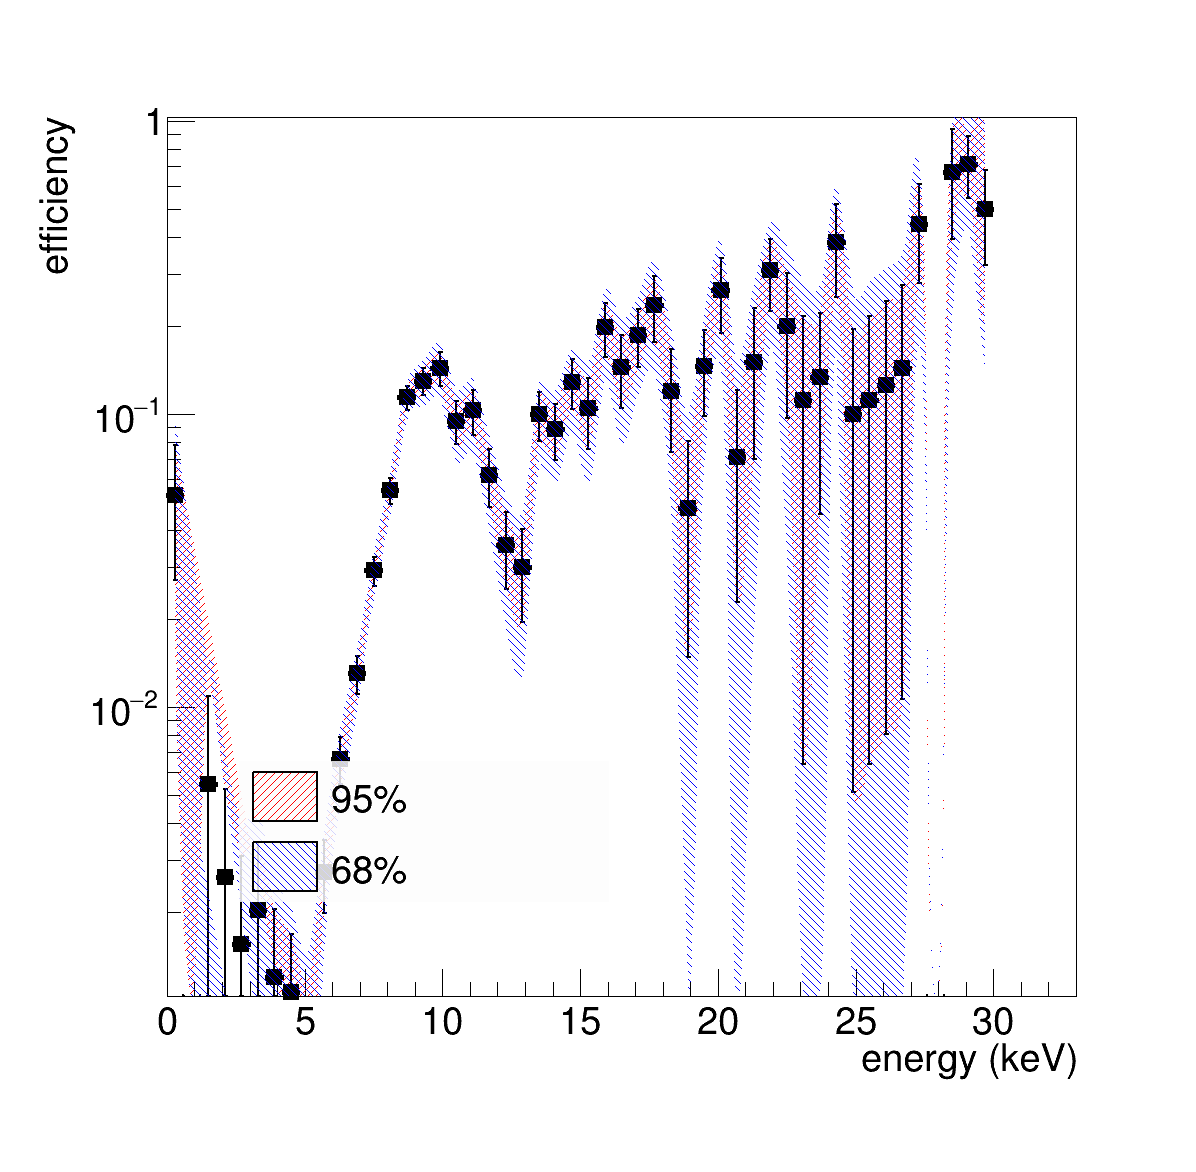
\includegraphics[width=0.45\linewidth]{effB.png}
  	\caption{Detection efficiency of Nuclear Recoil (NR) signals (left) and Electron Recoil (ER) signals (right) as a function of their reconstructed energy.}
  	\label{fig:effB}
\end{figure}


\begin{figure}[ht]
	\centering
	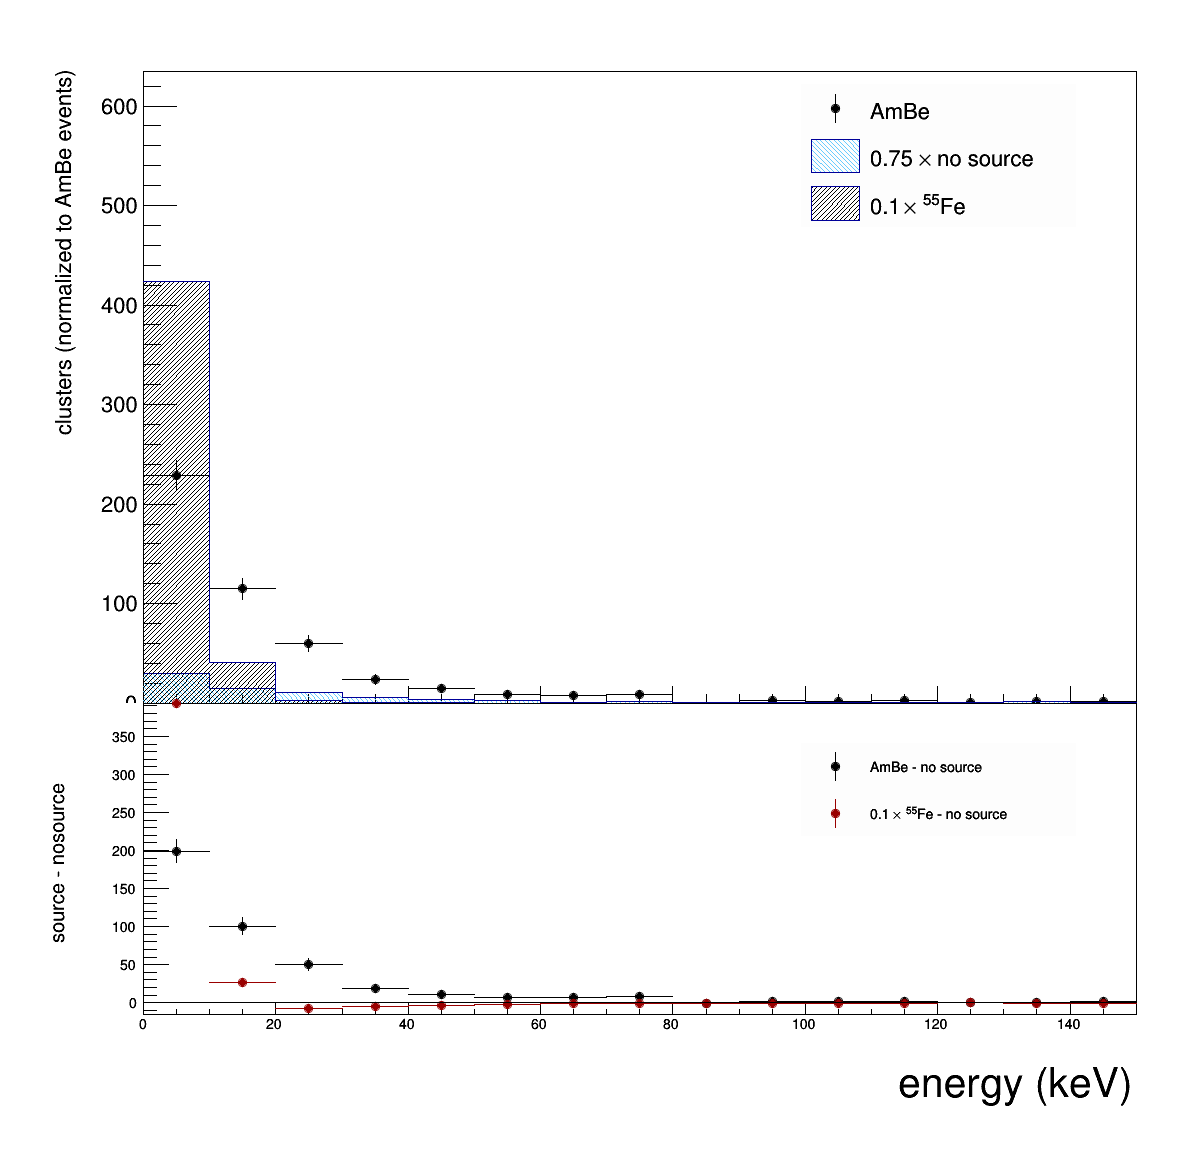
\includegraphics[width=0.45\linewidth]{energyExt.png}
	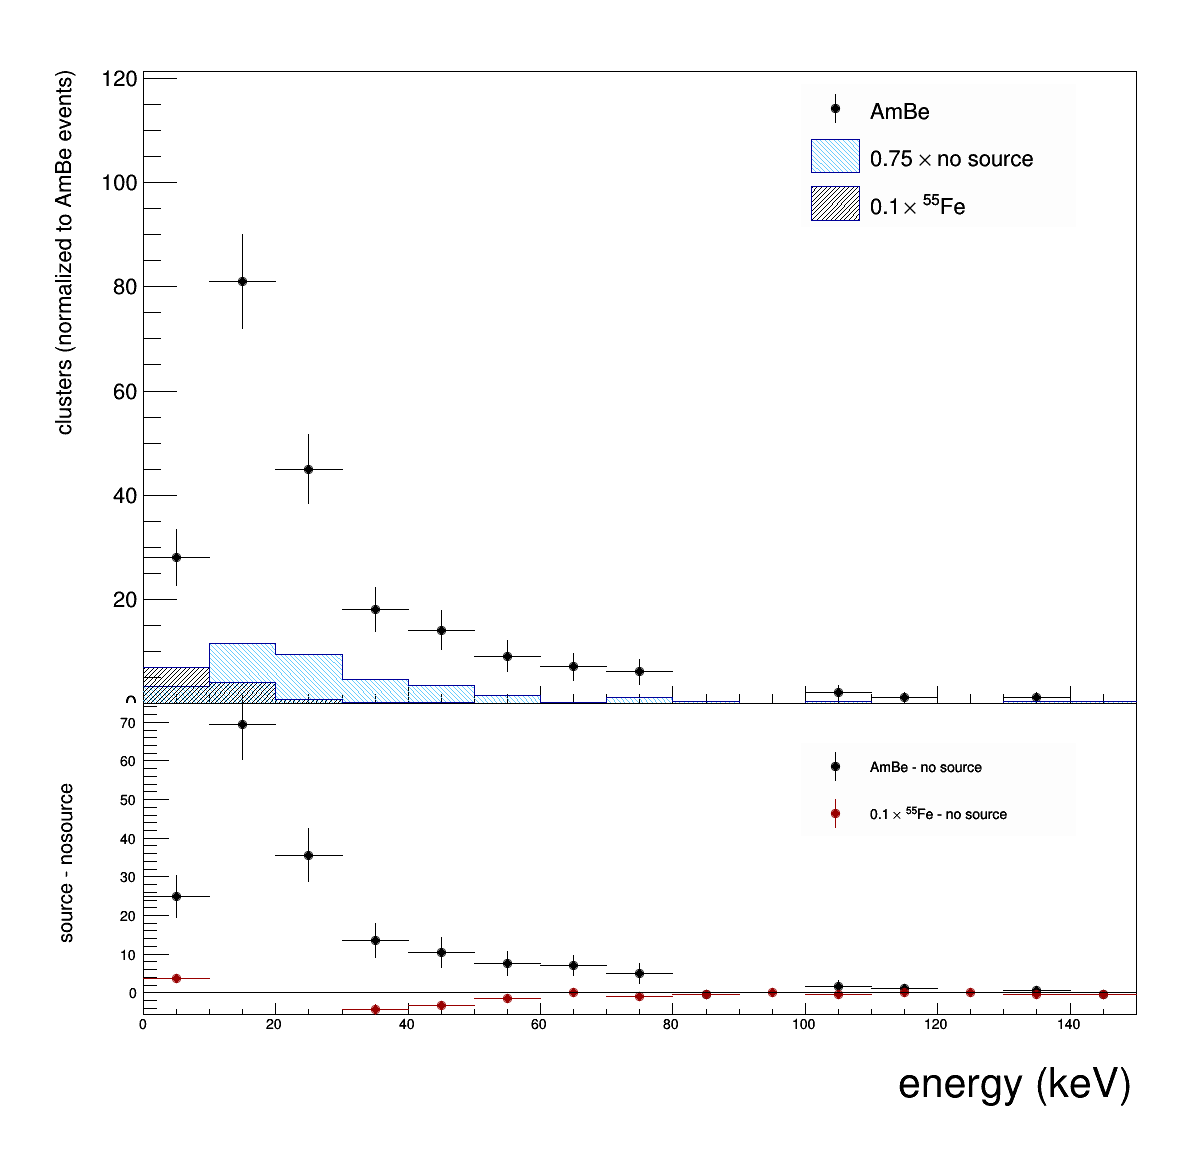
\includegraphics[width=0.45\linewidth]{energyExt_cut.png}
  	\caption{Spectra of energy of the clusters reconstructed in three different run types before (left) and after (right) cuts on energy densities.}
  	\label{fig:energy}
\end{figure}
\textcolor{red}{vogliamo provare a dimizzera la bin widt per gli spettri in energia?}
\begin{figure}[ht]
	\centering
	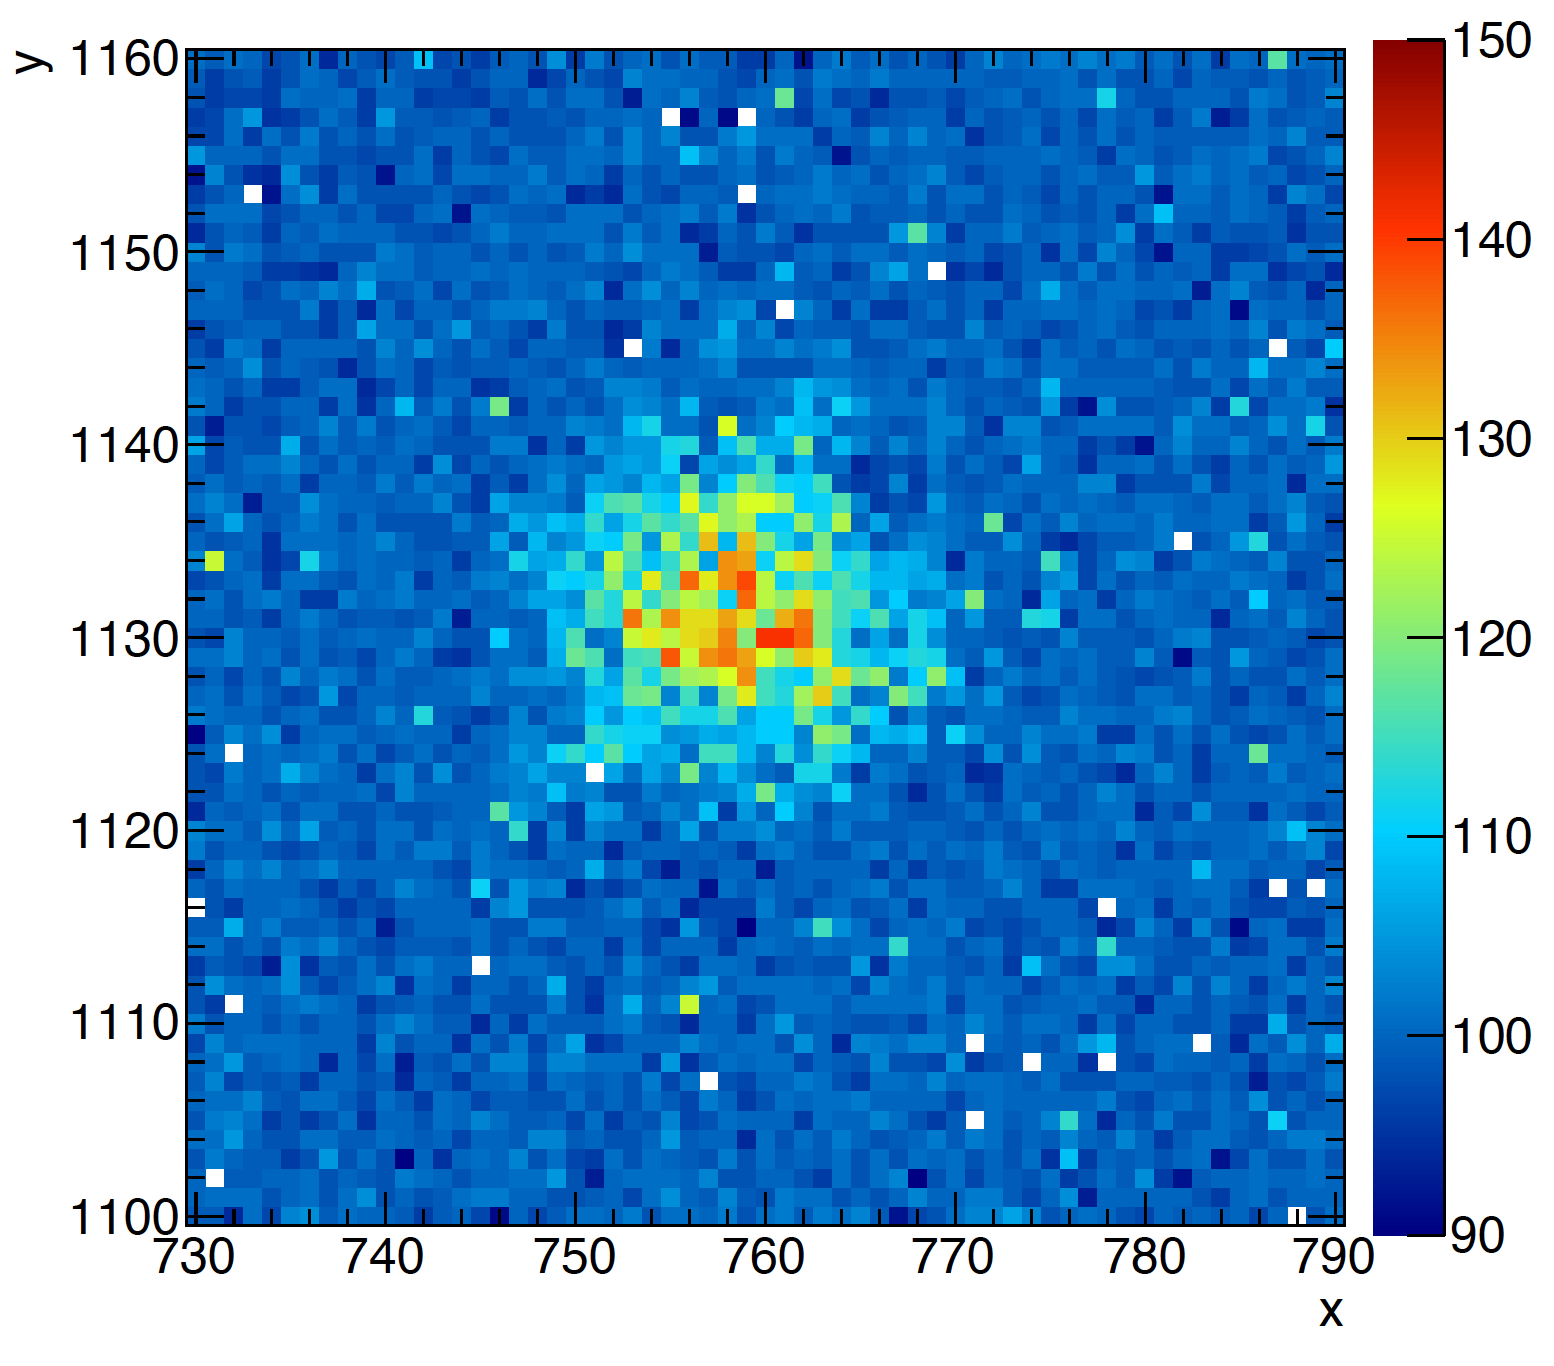
\includegraphics[width=0.50\linewidth]{granchio.png}
  	\caption{Example of a signal reconstructed as a Nuclear Recoil (NR) with an energy of 9~keV.}
  	\label{fig:granchio}
\end{figure}

\textcolor{red}{non farei vedere electron recoil che non ha senso in funzione dell'energia con questo campione }


\bibliography{mybiblio}{}
\bibliographystyle{ieeetr}

\end{document}

